\documentclass[10pt]{beamer}
\usetheme{Frankfurt}
\usepackage[utf8]{inputenc}
\usepackage[spanish,es-tabla]{babel}
\usepackage{amsmath}
\usepackage{amsfonts}
\usepackage{amssymb}
\usepackage{graphicx}
\graphicspath{{imagenes/}}									% Ruta de las imagenes, solo escribir nombre de la imagen
\author{Ciro Fabián Bermúdez Márquez}
\title{Síntesis de integradores de orden fraccionario usando hardware analógico reprogramable y su aplicación en un oscilador caótico}
%\setbeamercovered{transparent} 
%\setbeamertemplate{navigation symbols}{} 
%\logo{} 
\institute{Benemérita Universidad Autónoma de Puebla} \date{6 de Febrero de 2020} 
%\subject{}

%---------------------------------------------------------------------
%                      Paquetes adicionales                          %
%---------------------------------------------------------------------
\decimalpoint
\usepackage{xcolor}
\usepackage{ragged2e}
\usepackage{etoolbox}

\apptocmd{\frame}{}{\justifying}{} % Allow optional arguments after frame.

\setbeamertemplate{footline}
{
  \leavevmode%
  \hbox{%
  \begin{beamercolorbox}[wd=.333333\paperwidth,ht=2.5ex,dp=1ex,center]{author in head/foot}%
    \usebeamerfont{author in head/foot}Ciro Fabián Bermúdez Márquez
  \end{beamercolorbox}%
  \begin{beamercolorbox}[wd=.333333\paperwidth,ht=2.5ex,dp=1ex,center]{title in head/foot}%
    \usebeamerfont{title in head/foot}Benemérita Universidad Autónoma de Puebla
  \end{beamercolorbox}%
  \begin{beamercolorbox}[wd=.333333\paperwidth,ht=2.5ex,dp=1ex,right]{date in head/foot}%
    \usebeamerfont{date in head/foot}Facultad de Ciencias de la Electrónica\hspace*{2em}
    \insertframenumber{} / \inserttotalframenumber\hspace*{2ex} 
  \end{beamercolorbox}}%
  \vskip0pt%
}


%\usefonttheme{serif}
\usefonttheme[onlymath]{serif}



\setbeamertemplate{caption}[numbered]
\theoremstyle{definition}
	\newtheorem{defn}{Definición}
	\newtheorem{exmp}{Ejemplo}
	\newtheorem{law}{Ley}

\begin{document}
%%----------------------------------------------------------------------------------
%%----------------------------------------------------------------------------------
	\begin{frame}[plain]
	
		\begin{center}
			\textbf{Facultad de Ciencias de La Electrónica}
		\end{center}
		
		\begin{center}
			\textcolor{blue}{Benemérita Universidad Autónoma de Puebla}
		\end{center}
		
		\begin{figure}[hbtp]
			\centering
			
\includegraphics[width = 2.5cm]{logobuap.png} 
		\end{figure}
		
		\begin{center}
			\textbf{Licenciatura en Ingeniería Mecatrónica}
		\end{center}
						
		\begin{center}
			\begin{Large}
			\textcolor{blue}{Síntesis de integradores de orden fraccionario usando hardware analógico reprogramable y su aplicación en un oscilador caótico}
			\end{Large}
		\end{center}
		
		\begin{center}
			\textbf{Ciro Fabián Bermúdez Márquez }
		\end{center}
		
		\begin{center}
			\textbf{Asesor:} Dr. Jesús Manuel Muñoz Pacheco
		\end{center}
	\end{frame}
%%----------------------------------------------------------------------------------
%%----------------------------------------------------------------------------------
	\begin{frame}
		\tableofcontents
	\end{frame}
%%----------------------------------------------------------------------------------
%%----------------------------------------------------------------------------------
	\section{Introducción}
	\begin{frame}
		\frametitle{Introducción}
		\begin{block}{Cálculo fraccionario}
		\justifying
		El cálculo fraccionario es una generalización de la  diferenciación y la integración para ordenes no enteros del operador $_{a}D_{t}^{\alpha}$ con $\alpha \in \mathbb{R}$. \cite{Petras2011}
			\begin{figure}[!h]
				\begin{minipage}[c]{0.48\textwidth}
					\textbf{Ventajas}
					\begin{itemize}
								\justifying
								\item Describe y modela fenómenos físicos con mayor precisión.
								\item Poseen memoria de todos los eventos pasados.
								\item Es un área de oportunidad emergente.
					\end{itemize}
				\end{minipage} \hfill \begin{minipage}[c]{0.48\textwidth}
					\textbf{Desventajas}
					\begin{itemize}
								\justifying
								\item Implementar algoritmos de orden fraccional no es trivial.
								\item Implementación física compleja.
					\end{itemize}
				\end{minipage}
			\end{figure}		
		\end{block}
	\end{frame}
%%----------------------------------------------------------------------------------
%%----------------------------------------------------------------------------------	
	\begin{frame}
		\frametitle{Introducción}
		\begin{block}{Áreas de impacto}
		\begin{figure}[!h]
				\begin{minipage}[c]{0.48\textwidth}
					\begin{itemize}
								\justifying
								\item Física
								\item Electrónica
								\item Sistemas de control
								\item Robótica 
					\end{itemize}
				\end{minipage} \hfill \begin{minipage}[c]{0.48\textwidth}
					\begin{itemize}
								\justifying
								\item Procesamiento de señales
								\item Química
								\item Bio-ingeniería
								\item {\color{red} Teoría del caos}
					\end{itemize}
				\end{minipage}
			\end{figure}
		\end{block}
	\end{frame}		
%%----------------------------------------------------------------------------------
%%----------------------------------------------------------------------------------	
	\section{Objetivos}
	\begin{frame}
		\frametitle{Objetivos}
		\begin{block}{Objetivo general}
		\justifying
			Diseño e implementación electrónica de integradores de orden fraccionario mediante una expansión de fracciones continuas (CFE) para su aplicación en sistemas caóticos.
		\end{block}
		
		\begin{block}{Objetivos específicos}
			\begin{itemize}
			\justifying
				\item Analizar el método de expansión de fracciones continuas para generar una metodología de diseño en MATLAB.
				\item Caracterizar el error de la expansión de fracciones continuas para generar reglas de diseño.
				\item Diseñar e implementar en FPAA el integrador de orden fraccionario con aproximaciones de ordenes superiores.
				\item Diseñar e implementar de FPAA un oscilador caótico de orden fraccionario	
			\end{itemize}
		\end{block}
	\end{frame}
%%----------------------------------------------------------------------------------
%%----------------------------------------------------------------------------------	
	\section{Fundamentos teóricos}
	\begin{frame}
		\frametitle{Fundamentos teóricos}
		\begin{block}{Derivada fraccionaria}
		Definición de Grünwald–Letnikov.
			\begin{equation}
				D^{\alpha}_{t} f(t) = \lim_{h \to 0} \frac{1}{h^{\alpha}}   \sum_{j = 0}^{\infty} (-1)^{j} \binom{\alpha}{j} f(t - jh)
			\end{equation}
			
		Definición de Riemann-Louville.
			\begin{equation}
				D^{\alpha}_{t} f(t) = \frac{1}{\Gamma(n-\alpha)} \frac{d^{n}}{dt^{n}} \int_{0}^{t} \frac{f(\tau)}{(t-\tau)^{\alpha -n +1}} d\tau
			\end{equation}
		\end{block}
	\end{frame}
%%----------------------------------------------------------------------------------
%%----------------------------------------------------------------------------------	
	\begin{frame}
		\frametitle{Fundamentos teóricos}
		\begin{figure}[hbtp]
			\centering
			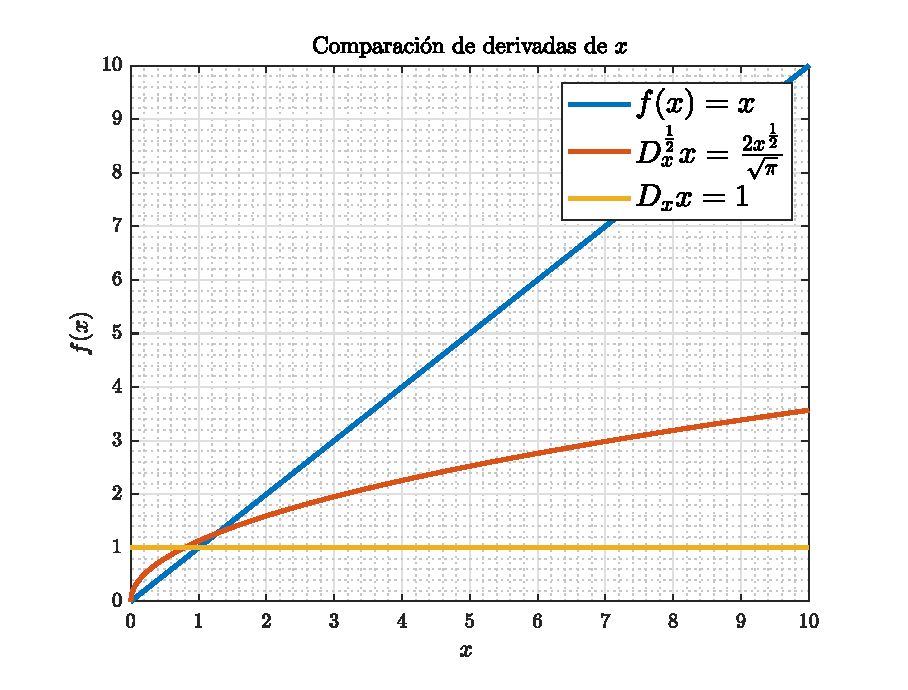
\includegraphics[width = 9cm]{A3_derivada_x.eps}
			\caption{Comparación de derivada entera y fraccionaria.}
		\end{figure}
	\end{frame}	
%%----------------------------------------------------------------------------------
%%----------------------------------------------------------------------------------
	\begin{frame}
		\frametitle{Fundamentos teóricos}
		\begin{block}{Transformada de Laplace de integrales y derivadas fraccionarias}
		\justifying
			La transformada de Laplace de la integral fraccionaria esta definida como:
			\begin{equation}
	 			\mathcal{L} \{ _{0}D_{t}^{-p} f(t) \} = s^{-p} F(s)
			\end{equation} 
			y dadas condiciones iniciales cero  la transformada de Laplace de la derivada fraccionaria de orden $r$ es:
			\begin{equation}
				\mathcal{L} \{ _{0}D_{t}^{r} f(t) \} = s^{r} F(s)
			\end{equation}
			respuesta de $20\alpha$ dB/década y 90 $\alpha$ deg.
		\end{block}
	\end{frame}	
%%----------------------------------------------------------------------------------
%%----------------------------------------------------------------------------------	
	\begin{frame}
		\frametitle{Fundamentos teóricos}
		\begin{block}{Expansión de fracciones continuas (CFE) definición}
		\justifying
			A una expresión de la forma:
				\begin{equation}
			a_{1} + \cfrac{b_{1}}{a_{2} + \cfrac{b_{2}}{a_{3} + \cfrac{b_{3}}{a_{4} + \genfrac{}{}{0pt}{0}{}{\ddots}}}}
			\label{ec:fracciones_cont}
		\end{equation} 
	se le conoce como una fracción continua. En general $a_{1},a_{2},a_{3},$ $\cdots$ $, b_{1}, b_{2}, b_{3}$ pueden ser cualquier número real o complejo, y el número de términos pueden ser finito o infinito.
	Una manera más conveniente de escribir la ecuación (\ref{ec:fracciones_cont}) es:
	\begin{equation}
		a_{1} + \frac{b_{1}}{a_{2} } \genfrac{}{}{0pt}{0}{}{+}   \frac{b_{2}}{a_{3}}  \genfrac{}{}{0pt}{0}{}{+}  \frac{b_{3}}{a_{4}}  \genfrac{}{}{0pt}{0}{}{+}  \genfrac{}{}{0pt}{0}{}{\cdots} 
		\label{ec:fracciones_cont_sim}
	\end{equation}
		\end{block}
	\end{frame}
%%----------------------------------------------------------------------------------
%%----------------------------------------------------------------------------------	
	\begin{frame}
		\frametitle{Fundamentos teóricos}
		\begin{block}{Lagrange 1776 CFE de $(1 + x)^{\alpha}$}
		Si consideramos:
			\begin{scriptsize}
				\begin{equation}
					x = s-1
				\end{equation}
			\end{scriptsize}
			\begin{scriptsize}
				\begin{equation}
				{\color{blue} 
		 			(1 + x)^{\alpha} = \frac{1}{1} \genfrac{}{}{0pt}{0}{}{-} \frac{\alpha x}{1} \genfrac{}{}{0pt}{0}{}{+} \frac{\frac{1(1 + \alpha)}{1\cdot2}\,x}{1} \genfrac{}{}{0pt}{0}{}{+} \frac{\frac{1(1 - \alpha)}{2\cdot3}\,x}{1} \genfrac{}{}{0pt}{0}{}{+} \frac{\frac{2(2 + \alpha)}{3\cdot4}\,x}{1} \genfrac{}{}{0pt}{0}{}{+} \frac{\frac{2(2 - \alpha)}{4\cdot5}\,x}{1} \genfrac{}{}{0pt}{0}{}{+} \genfrac{}{}{0pt}{0}{}{\cdots} }
				\label{ec:lagrange_conv}
				\end{equation}
			\end{scriptsize}	
			
		La ecuación (\ref{ec:cfe_inutil}) es la encontrada en múltiples artículos:
			\begin{scriptsize}
				\begin{equation}
				{\color{red} 
			 		(1 + x)^{\alpha} = \frac{1}{1}  \genfrac{}{}{0pt}{0}{}{-} \frac{\alpha x}{1} \genfrac{}{}{0pt}{0}{}{+} \frac{(1 + \alpha)x}{2} \genfrac{}{}{0pt}{0}{}{+} \frac{(1 - \alpha)x}{3} \genfrac{}{}{0pt}{0}{}{+} \frac{(2 + \alpha)x}{2} \genfrac{}{}{0pt}{0}{}{+} \frac{(2-\alpha)x}{5} \genfrac{}{}{0pt}{0}{}{+} \genfrac{}{}{0pt}{0}{}{\cdots} }
			 		\label{ec:cfe_inutil}
				\end{equation}
			\end{scriptsize}	
		\end{block}
	\end{frame}
%%----------------------------------------------------------------------------------
%%----------------------------------------------------------------------------------	
	\begin{frame}
		\frametitle{Fundamentos teóricos}
		\begin{block}{Algoritmo propuesto}
		\justifying
		El $n$-ésimo término de la expansión de fracciones continuas para la ecuación (\ref{ec:lagrange_conv}) se puede calcular utilizando la siguiente ecuación:
			\begin{equation}
				\frac{\psi(n) \left[ \psi(n) + (-1)^{n} \alpha \right]}{(n-1)n}
				\label{ec:calculo_terminos_cfe}
			\end{equation}
	donde la función $\psi(x)$ para $x\geq2$, $x\in \mathbb{Z}^{+}$ esta definida como\footnote{$\left\lfloor x\right\rfloor$ es  la función redondeo hacia el entero inferior anterior.}:
				\begin{equation}
					\psi(x) = \left\lfloor \frac{x}{2}\right\rfloor
				\end{equation}
		\end{block}
	\end{frame}		
%%----------------------------------------------------------------------------------
%%----------------------------------------------------------------------------------	
	\begin{frame}
		\frametitle{Fundamentos teóricos}
			\lstinputlisting[style = MATLAB, caption =  Función cfetf, label = cod:cfetf]{../codigos/cfetf.m}
	\end{frame}		
%%----------------------------------------------------------------------------------
%%----------------------------------------------------------------------------------	
	\begin{frame}
		\frametitle{Fundamentos teóricos}
		\begin{block}{Aproximación de primer y segundo orden de la CFE}
		\justifying
			La aproximación para un integrador fraccionario $\frac{1}{s^{\alpha}}$ para primer y segundo orden tienen la forma:
			\vspace{0.25cm}
			\begin{equation}
				\genfrac{}{}{0pt}{0}{}{_{(c_{2})}} \frac{1}{s^{\alpha}} \approx \frac{(1 - \alpha)s + (1 + \alpha) }{(1 + \alpha)s + (1 - \alpha)} 
			\end{equation}
			\vspace{0.25cm}
			\begin{equation}
		\genfrac{}{}{0pt}{0}{}{_{(c_{4})}} \frac{1}{s^{\alpha}} \approx \frac{(\alpha^{2} - 3\alpha + 2) s^{2} + (8 - 2 \alpha^{2})s + (\alpha^{2} + 3\alpha + 2) }{(\alpha^{2} + 3\alpha + 2) s^{2} + (8 - 2 \alpha^{2})s + (\alpha^{2} - 3\alpha + 2)}
	\end{equation}
		\end{block}
	\end{frame}	
%%----------------------------------------------------------------------------------
%%----------------------------------------------------------------------------------	
	\begin{frame}
		\frametitle{Fundamentos teóricos}
		\begin{block}{Ejemplo}
			\begin{scriptsize}
			\begin{table}[!hbp]
		\caption{Aproximaciones racionales de $\frac{1}{s^{0.5}}$}
		\label{tab:aprox_cfe_alpha_0.5}
		\centering
%		\resizebox{\textwidth}{!}{
		\begin{tabular}{c c c}
			\hline
			\textbf{Orden} &  \textbf{No. de términos} & \textbf{Aproximación racional}\\
			\hline
			$1$ 		& $2$ 		&  $\cfrac{s + 3}{3s + 1}$\\
					 		& 		 		& \\
			$2$			& $4$ 		&  $\cfrac{s^{2} + 10s + 5}{5 s^{2} + 10s + 1}$\\
							& 		 		& \\
			$3$ 		& $6$ 		&  $\cfrac{s^{3} + 21s^{2} + 35s + 7}{7 s^3 + 35 s^2 + 21 s + 1}$	\\
							& 		 		& \\
			$4$ 		& $8$ 		&  $\cfrac{s^4 + 36 s^3 + 126 s^2 + 84 s + 9}{9 s^4 + 84 s^3 + 126 s^2 + 36 s + 1}$\\
							& 		 		& \\
			$5$ 		& $10$ 		&  $\cfrac{s^5 + 55 s^4 + 330 s^3 + 462 s^2 + 165 s + 11}{11 s^5 + 165 s^4 + 462 s^3 + 330 s^2 + 55 s + 1}$\\
							& 		 		& \\
			\hline
		\end{tabular}
%		}
	\end{table}
			\end{scriptsize}
		\end{block}
	\end{frame}	
%%----------------------------------------------------------------------------------
%%----------------------------------------------------------------------------------	
	\begin{frame}
		\frametitle{Fundamentos teóricos}
		\begin{figure}[hbtp]
			\caption{Diagramas de bode comparativos de integrador fraccionario $\alpha = 0.5$.} 
			\label{fig:F1_bode_integrador_alpha05}
			\centering
			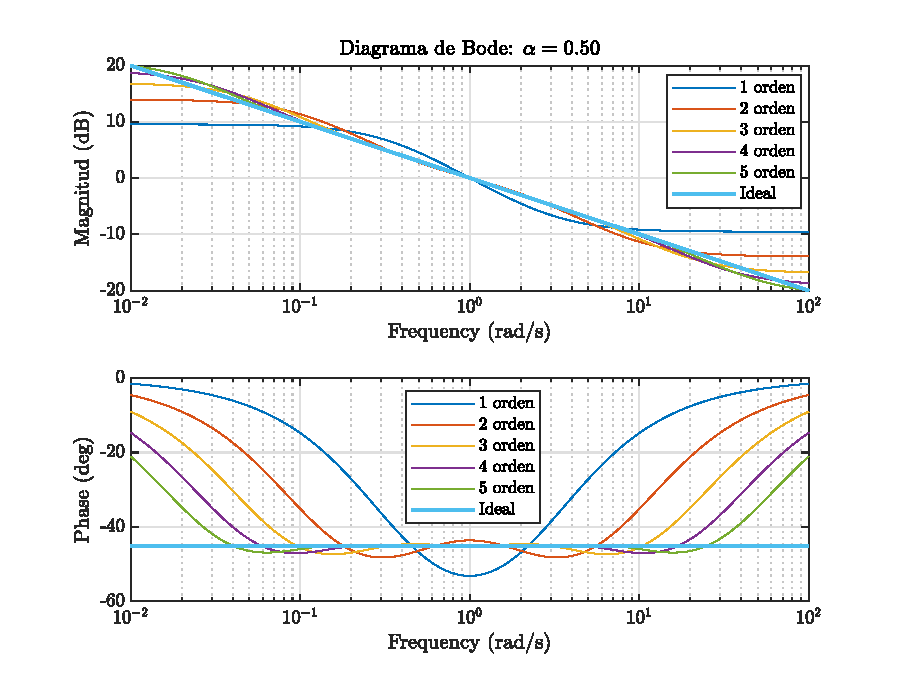
\includegraphics[width=9cm]{../imagenes/F1_bode_integrador_alpha05.eps}
		\end{figure}	
	\end{frame}
%%----------------------------------------------------------------------------------
%%----------------------------------------------------------------------------------	
	\begin{frame}
		\frametitle{Fundamentos teóricos}
		\begin{block}{Análisis de error de la CFE}
		\begin{small}
		\begin{equation}
			\mathrm{error}_{\mathrm{dB}} = 20\log_{10} \left| \frac{H(j\omega)}{G(j\omega)} \right|
			\label{ec:error_sin_norm}
		\end{equation}
	
		\begin{equation}
			\mathrm{error}_{\mathrm{deg}} = \phase{H(j\omega)} - \phase{G(j\omega)}
		\end{equation}
		
		\begin{equation}
			\mathrm{error}_{\mathrm{norm\,\,de\,\,mag}} = \cfrac{ 20\log_{10} \left| \frac{H(j\omega)}{G(j\omega)} \right| }{20 \alpha} = \cfrac{ \log_{10} \left| \frac{H(j\omega)}{G(j\omega)} \right| }{ \alpha}
		\end{equation}
	
		\begin{equation}
			\mathrm{error}_{\mathrm{norm\,\,de\,\,fase}} = \cfrac{\phase{H(j\omega)} - \phase{G(j\omega)}}{90\alpha}
		\end{equation}
		\end{small}
		\justifying
		donde $H(j\omega)$ es el integrador ideal $\frac{1}{s^{\alpha}}$ y $G(j\omega)$ es la función de transferencia aproximada del integrador utilizando CFE $ _{(c_{n})} \frac{1}{s^{\alpha}}$. 
		\end{block}
	\end{frame}		
%%----------------------------------------------------------------------------------
%%----------------------------------------------------------------------------------
	\begin{frame}
		\frametitle{Fundamentos teóricos}
		\begin{figure}[hbtp]
			\caption{Magnitud normalizada.}
			\centering
			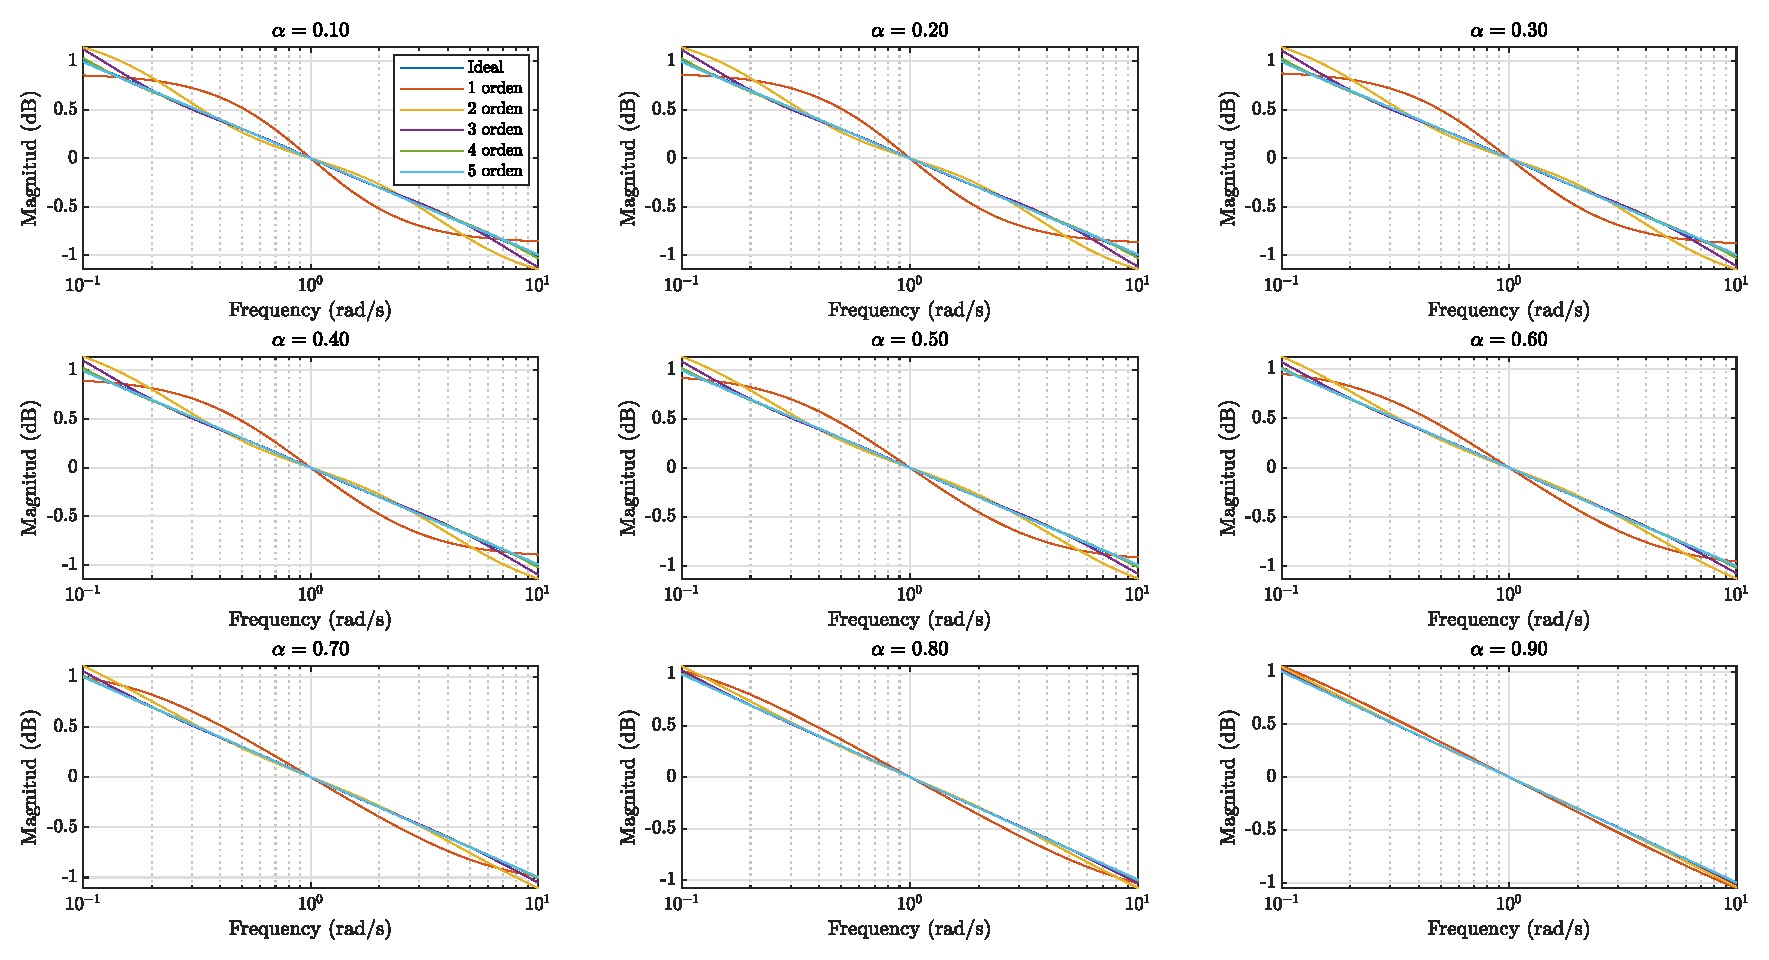
\includegraphics[trim={0cm 0cm 0cm 0.2cm},clip,width=1.3\textheight]{../imagenes/F6_bode_magnitud_norm_c.eps}
			% <left> <lower> <right> <upper>
		\end{figure}
	\end{frame}	
%%----------------------------------------------------------------------------------
%%----------------------------------------------------------------------------------	
	\begin{frame}
		\frametitle{Fundamentos teóricos}
		\begin{figure}[hbtp]
			\caption{Fase normalizada.}
			\centering
			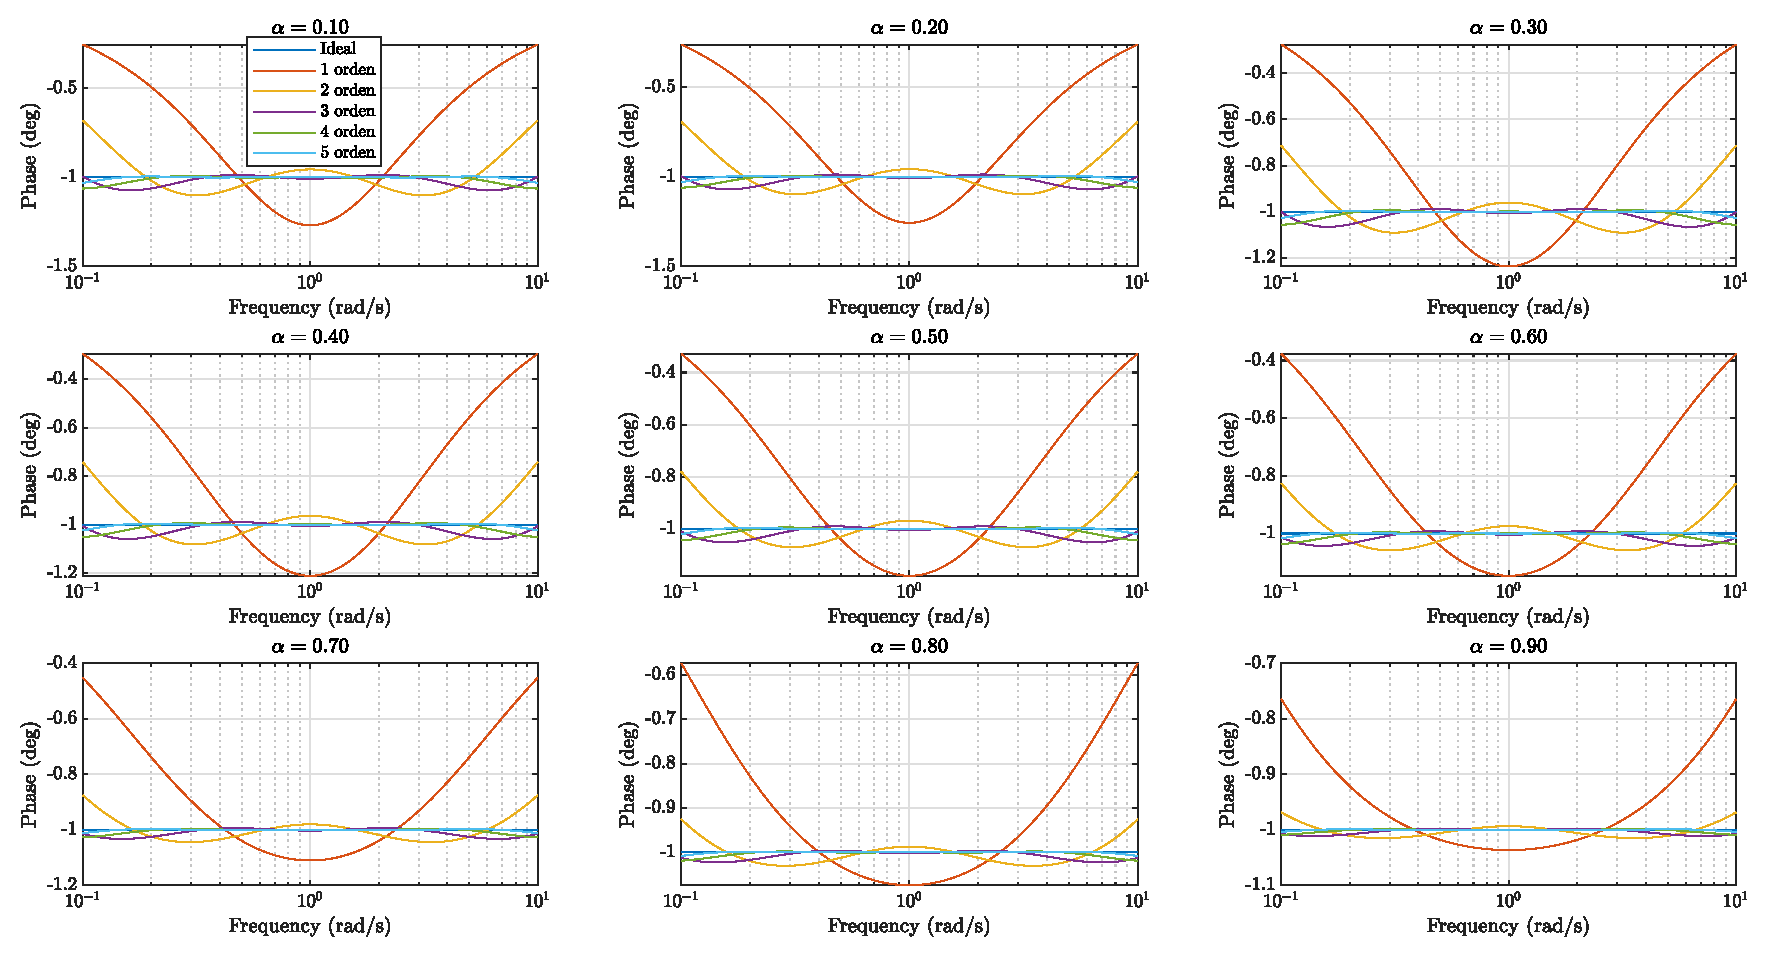
\includegraphics[trim={0cm 0cm 0cm 0.2cm},clip,width=1.3\textheight]{../imagenes/F7_bode_fase_norm_c.eps}
			% <left> <lower> <right> <upper>
		\end{figure}
	\end{frame}	
%%----------------------------------------------------------------------------------
%%----------------------------------------------------------------------------------
	\begin{frame}
		\frametitle{Fundamentos teóricos}
		\begin{figure}[hbtp]
			\caption{Error magnitud normalizado.}
			\centering
			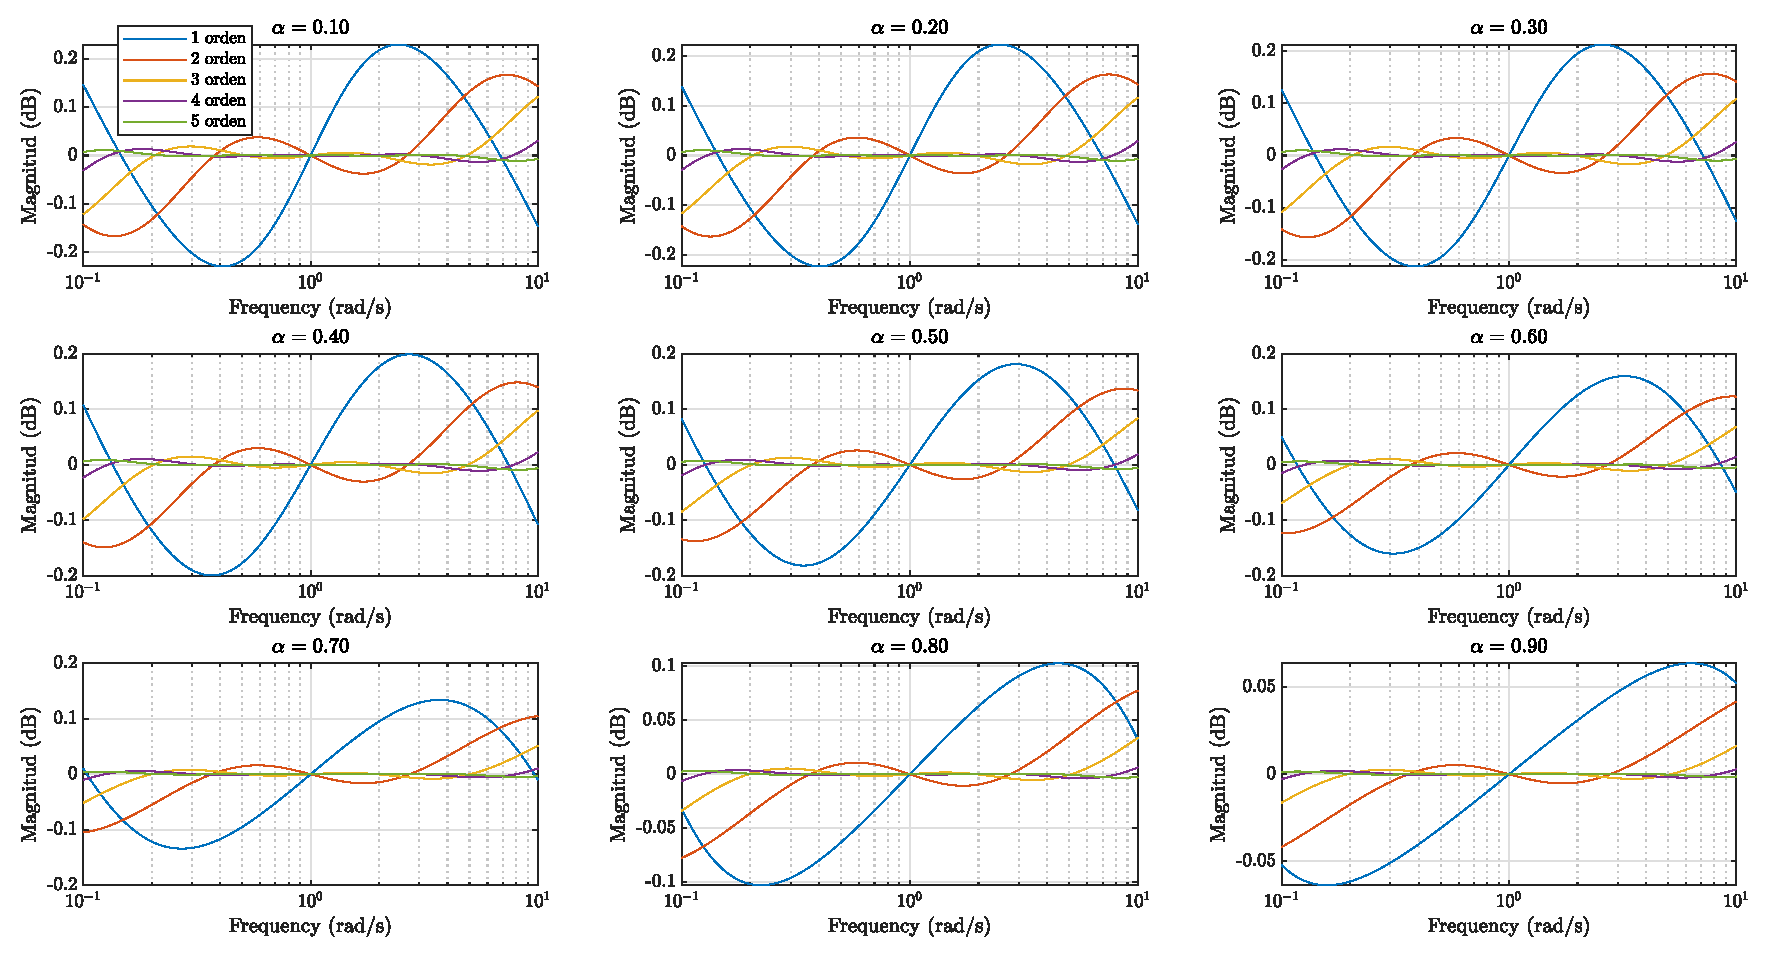
\includegraphics[trim={0cm 0cm 0cm 0.2cm},clip,width=1.3\textheight]{../imagenes/F8_bode_error_mag_norm_c.eps}
			% <left> <lower> <right> <upper>
		\end{figure}
	\end{frame}	
%%----------------------------------------------------------------------------------
%%----------------------------------------------------------------------------------	
	\begin{frame}
		\frametitle{Fundamentos teóricos}
		\begin{figure}[hbtp]
			\caption{Error fase normalizado.}
			\centering
			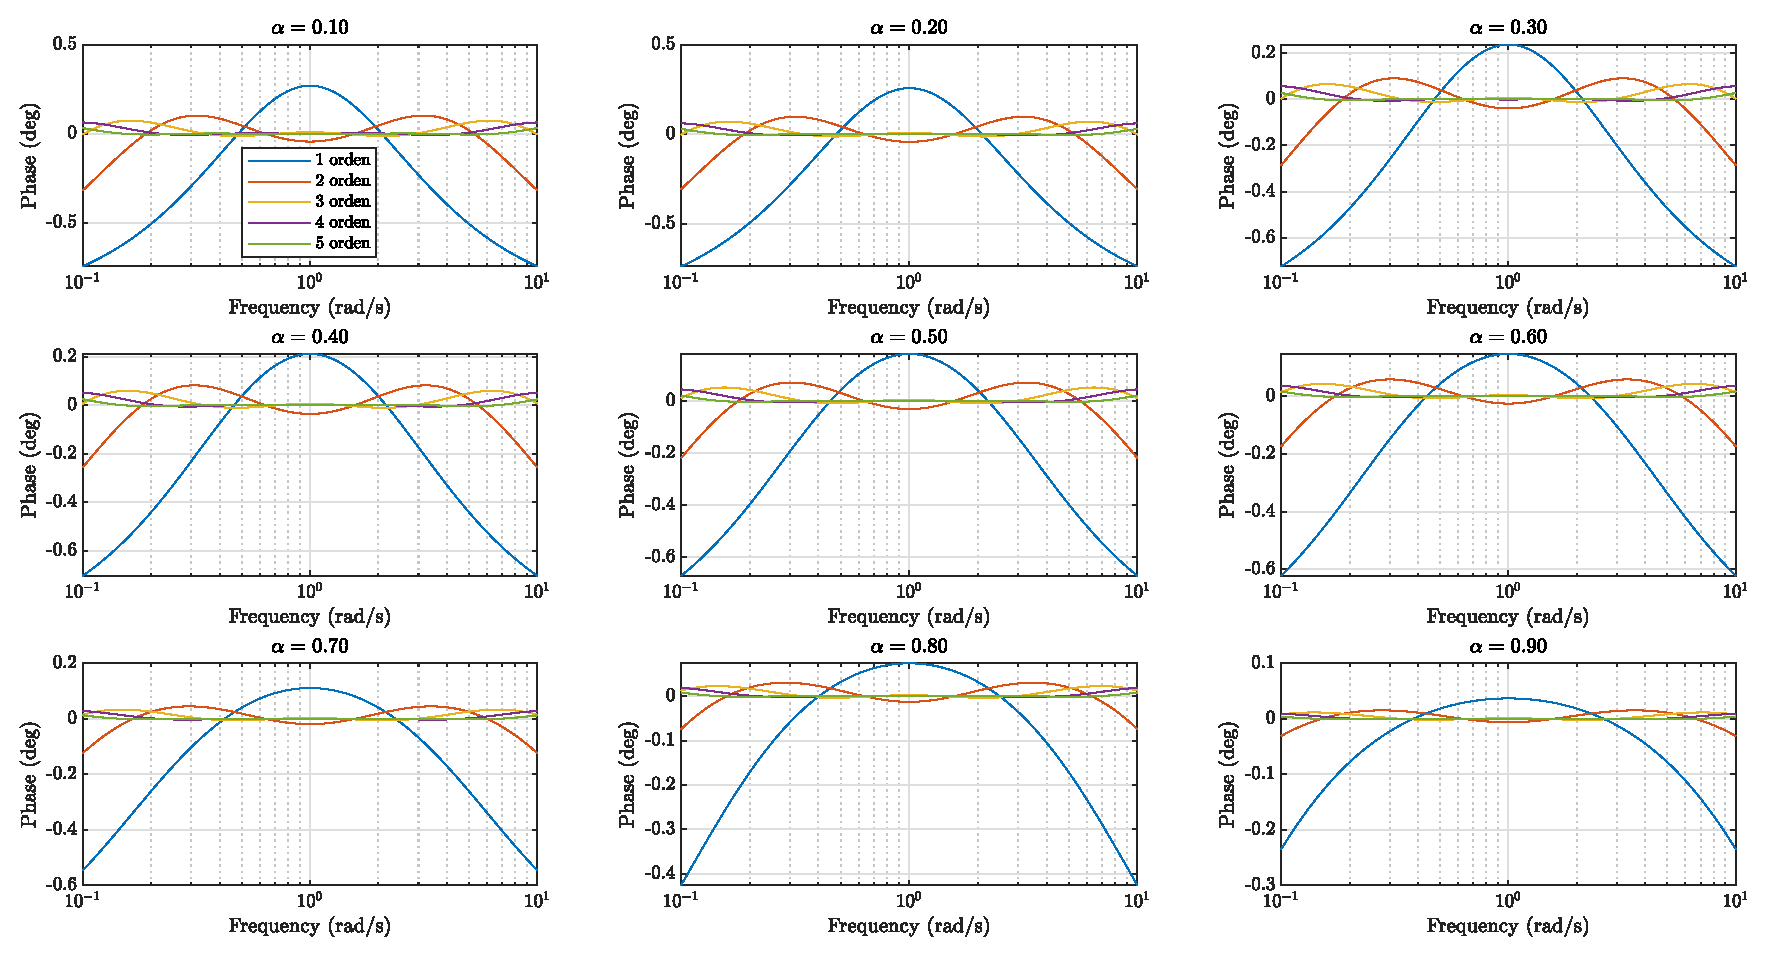
\includegraphics[trim={0cm 0cm 0cm 0.2cm},clip,width=1.3\textheight]{../imagenes/F9_bode_error_fase_norm_c.eps}
			% <left> <lower> <right> <upper>
		\end{figure}
	\end{frame}	
%%----------------------------------------------------------------------------------
%%----------------------------------------------------------------------------------
	\begin{frame}
		\frametitle{Fundamentos teóricos}
		\begin{block}{Análisis}	
		 \begin{center}
		 	\textbf{El porcentaje de error es mayor cuanto más pequeño sea $\alpha$}
		 \end{center}
		\begin{small}
		\vspace{-0.3cm}
		\begin{table}[!ht]                                 
		\centering            
		\caption{Promedio de error absoluto de magnitud normalizado en \% variando $\alpha$ y orden de función de transferencia.}                           
		\label{tab:prom_error_mag_norm}                               
			\begin{tabular}{cccccc}
				\hline                                             
				$\,\,\,\,\bm{\alpha}$\textbf{/Orden} & \textbf{1$^{\mathrm{er}}$} & \textbf{2$^{\mathrm{do}}$} & \textbf{3$^{\mathrm{er}}$} & \textbf{4$^{\mathrm{to}}$} & \textbf{5$^{\mathrm{to}}$} \\                     
				\hline                                             
				0.1 & 13.4397 & 7.5755 & 2.4058 & 0.5407 & 0.2754 \\
				                                         
				0.2 & 13.1089 & 7.3398 & 2.2960 & 0.5155 & 0.2639 \\
				                                              
				0.3 & 12.5614 & 6.9432 & 2.1189 & 0.4751 & 0.2454 \\
				                                            
				0.4 & 11.8034 & 6.3812 & 1.8827 & 0.4217 & 0.2203 \\
				                                            
				0.5 & 10.8454 & 5.6502 & 1.5991 & 0.3580 & 0.1897 \\
				                                           
				0.6 & 9.7075 & 4.7507 & 1.2822 & 0.2875 & 0.1548 \\ 
				                                         
				0.7 & 8.4275 & 3.6945 & 0.9478 & 0.2133 & 0.1168 \\ 
				                                              
				0.8 & 6.8606 & 2.5119 & 0.6123 & 0.1387 & 0.0772 \\ 
				                                             
				0.9 & 4.2249 & 1.2563 & 0.2916 & 0.0667 & 0.0377 \\ 
				\hline                                             
			\end{tabular}                                                             
		\end{table}
		\end{small}
		\end{block}
	\end{frame}	
%%----------------------------------------------------------------------------------
%%----------------------------------------------------------------------------------
	\section{Implementación de integradores fraccionarios}
	\begin{frame}
		\frametitle{Implementación de integradores fraccionarios}
		\begin{block}{¿Qué es una FPAA?}
			\begin{enumerate}
				\item Field Programmable Analog Arrays.
				\item Es un dispositivo analógico equivalente a las FPGA.
				\item QuadApex Develovment Board v2.0
				\item CAM (Configurable Analog Module)
				\item AnadigmDesigner2
			\end{enumerate}
		\end{block}
	\end{frame}
%%----------------------------------------------------------------------------------
%%----------------------------------------------------------------------------------	
	\begin{frame}
		\frametitle{Implementación de integradores fraccionarios}
			\begin{figure}[hbtp]
			\caption{Metodología de conexiones.}
			\centering
			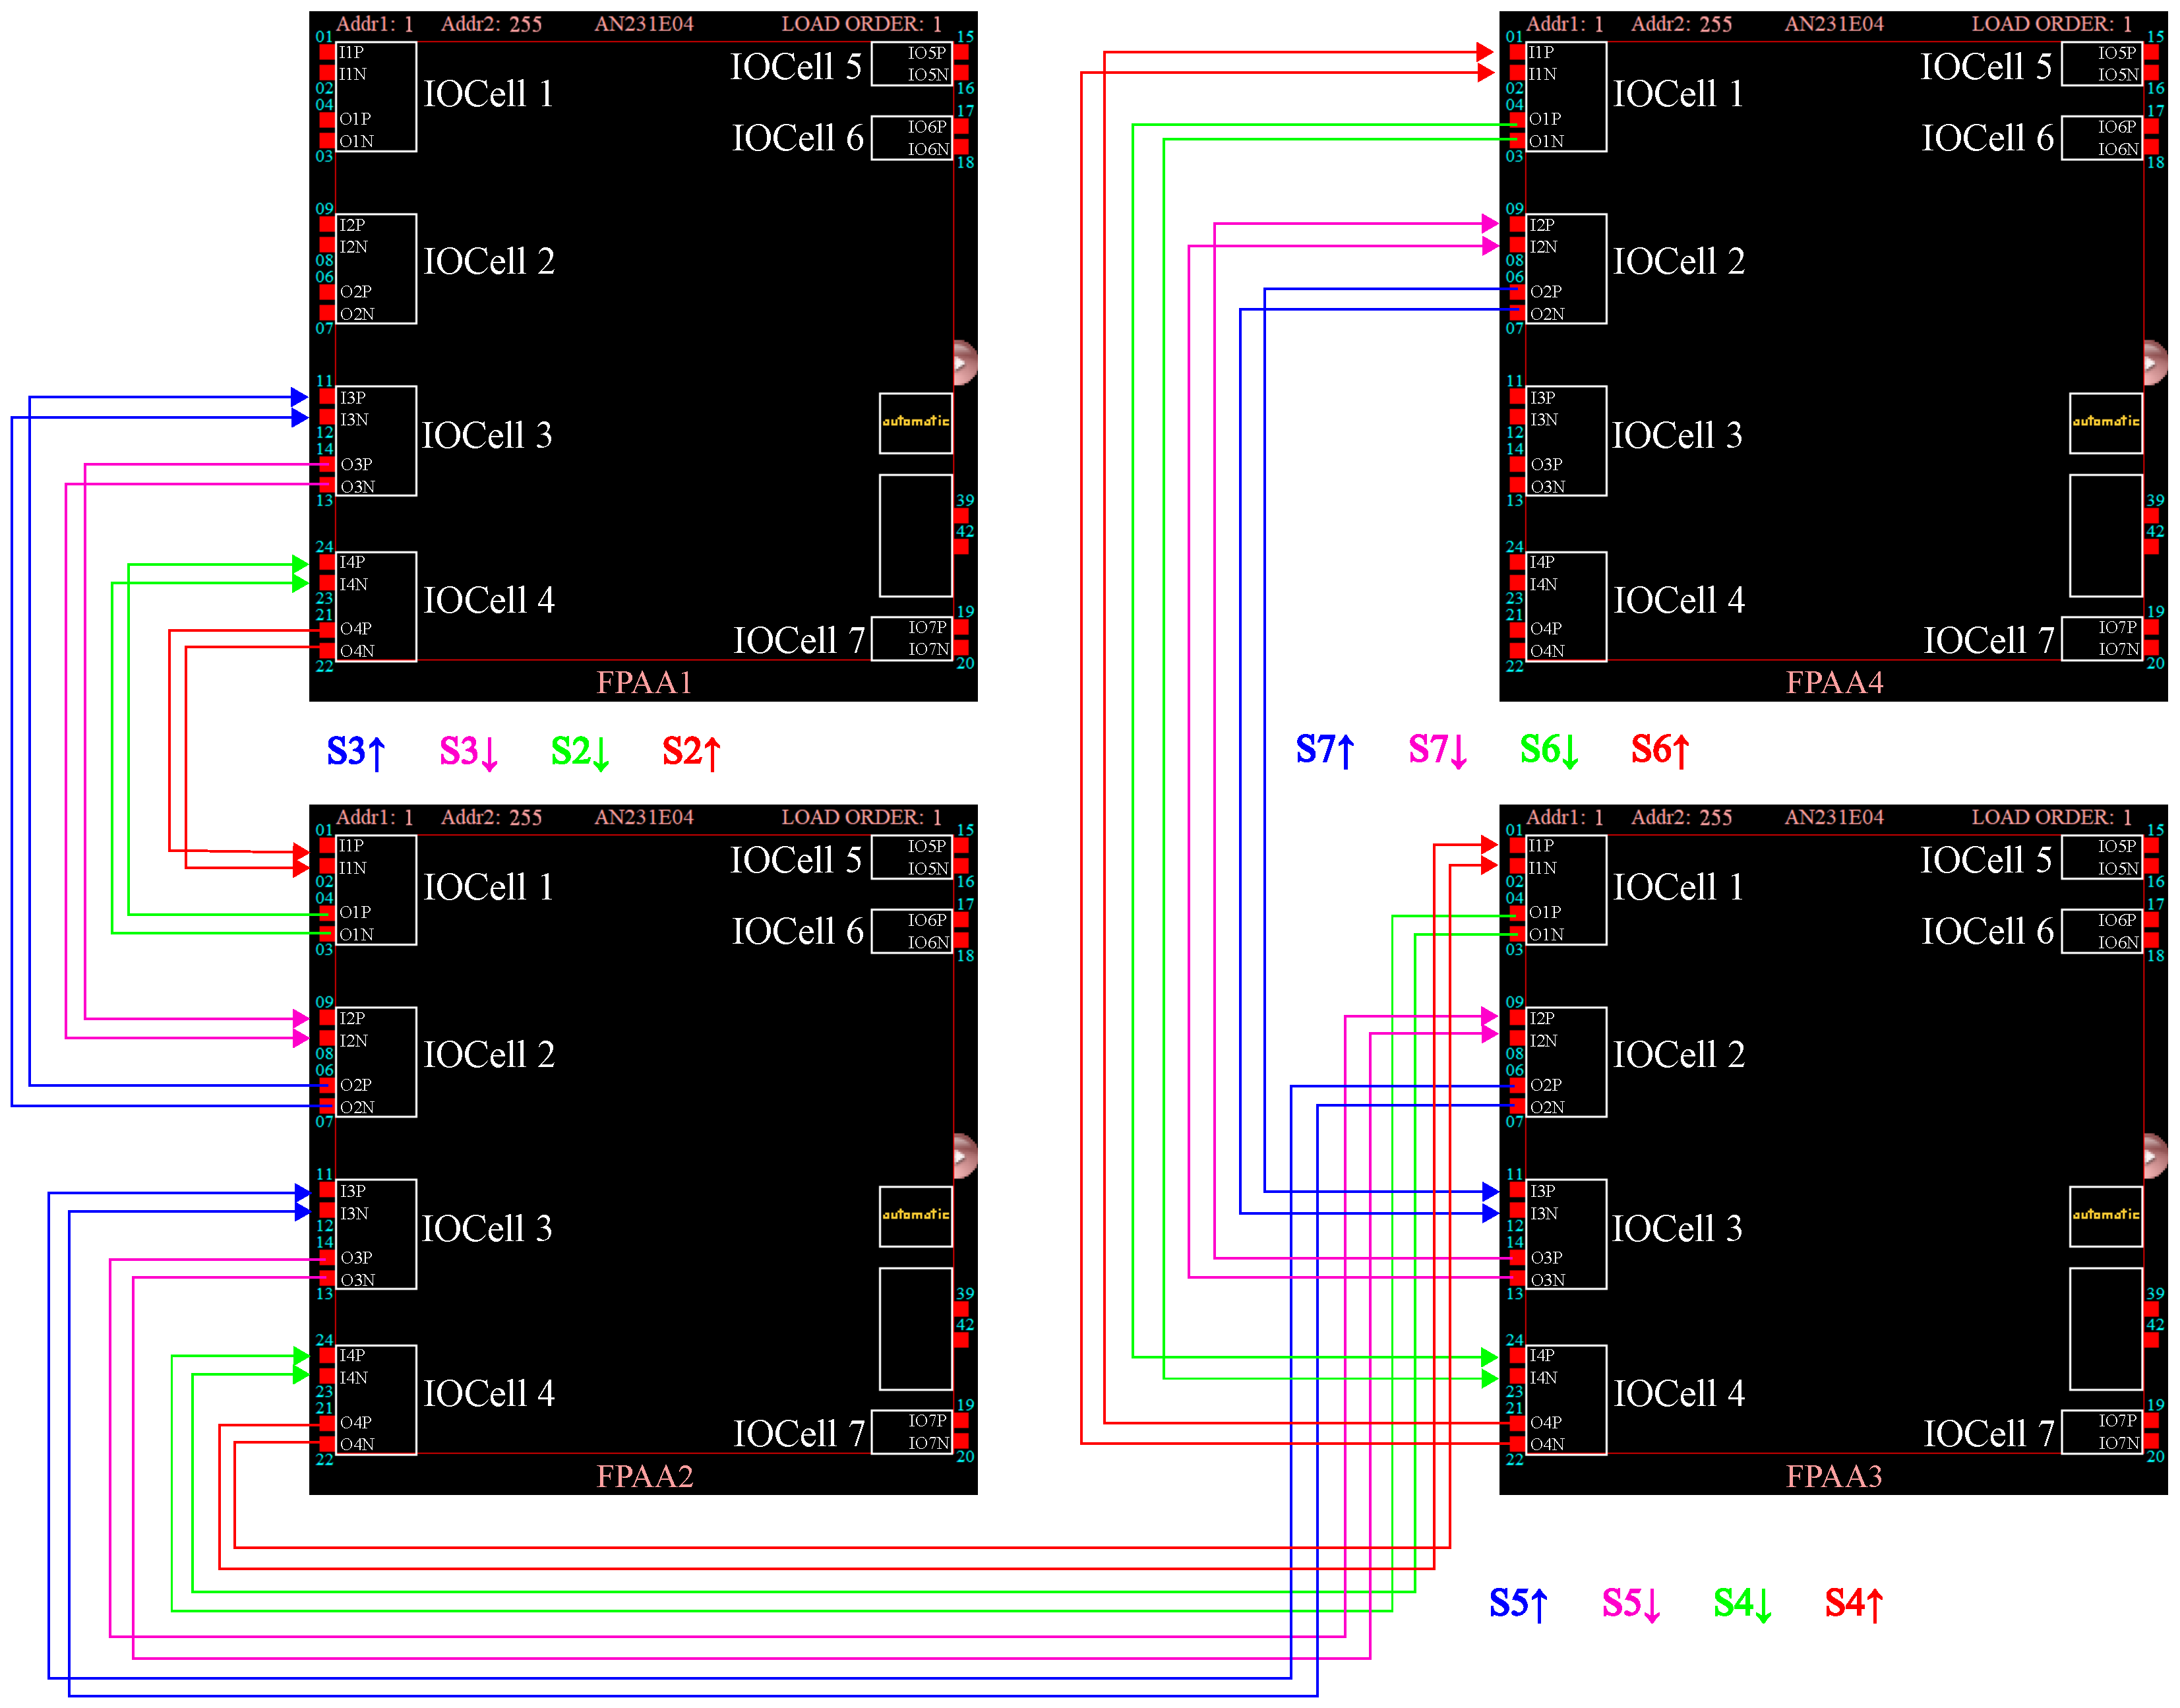
\includegraphics[width=0.8\textheight]{../imagenes/X6_conexiones_AD2.eps}
			% <left> <lower> <right> <upper>
			\end{figure}
	\end{frame}
%%----------------------------------------------------------------------------------
%%----------------------------------------------------------------------------------	
	\begin{frame}
		\frametitle{Implementación de integradores fraccionarios}
		\begin{block}{Configuración de relojes}
		El diseño se basa en seleccionar correctamente las frecuencias de reloj.
		\begin{equation}
			\mathrm{Sys1} = \frac{f_{c}}{m} \qquad \mathrm{Sys2} = \frac{f_{c}}{m}
			\label{ec:sys_clock}
		\end{equation}
		
		\begin{equation}
		\mathrm{Clock\,} h = \frac{\mathrm{Sys1}}{n}	\qquad   \mathrm{Clock\,} h = \frac{\mathrm{Sys2}}{n}
		\label{ec:clock_h}
		\end{equation}
		\justifying
		donde la frecuencia de reloj principal $f_{c}$ = 16 MHz y donde $n,m\in[1,510]$.
		\end{block}
	\end{frame}
%%----------------------------------------------------------------------------------
%%----------------------------------------------------------------------------------
	\begin{frame}
		\frametitle{Implementación de integradores fraccionarios}
		\begin{figure}[hbtp]
			\centering
			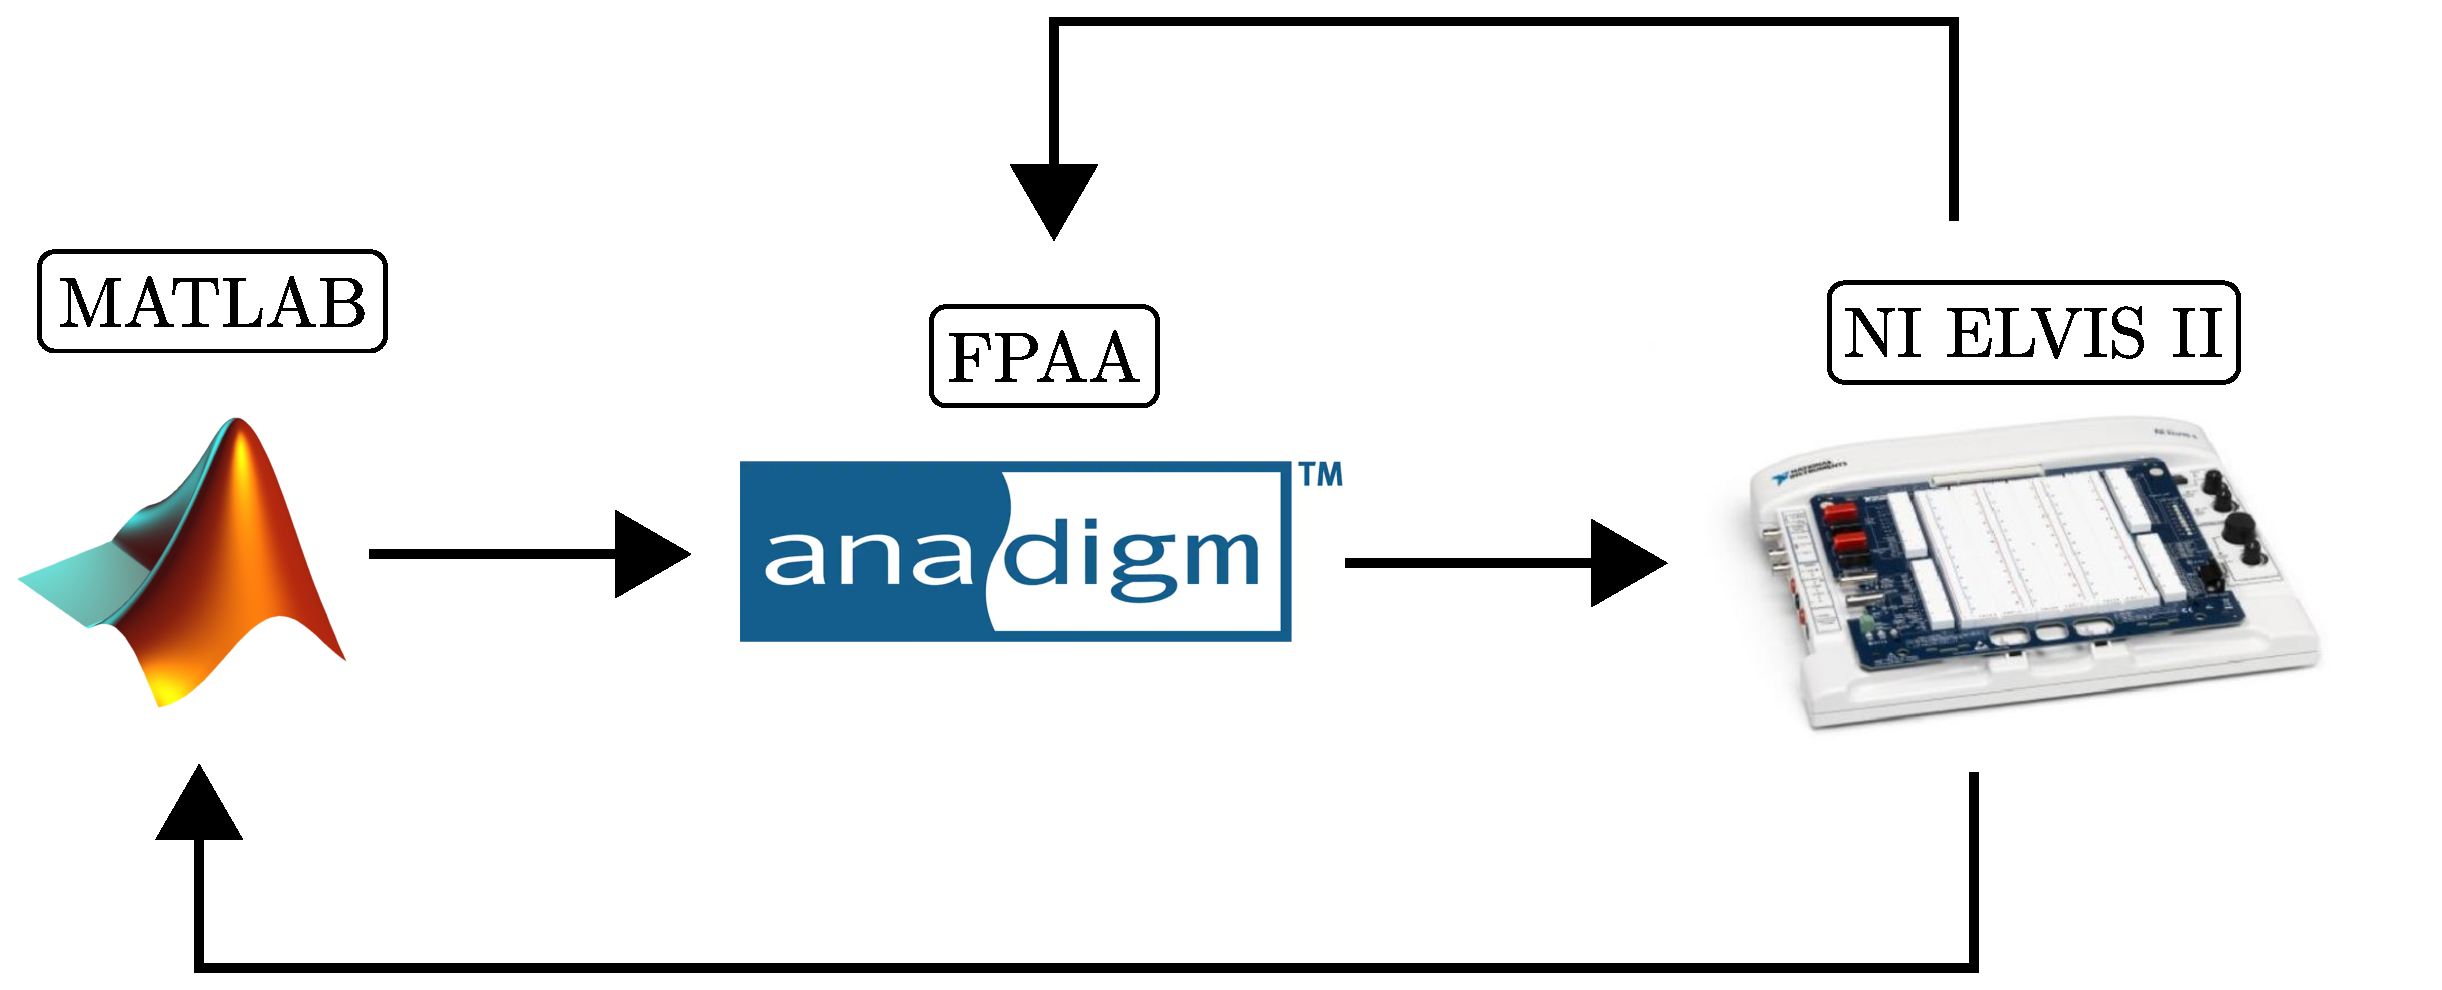
\includegraphics[width = 12cm]{descripcion.eps}
		\end{figure}
	\end{frame}
%%----------------------------------------------------------------------------------
%%----------------------------------------------------------------------------------
	\begin{frame}
		\frametitle{Implementación de integradores fraccionarios}
		\begin{block}{Configuración bilineal polo y cero}
		\textbf{CAM FilterBilinear}
			\begin{equation}
		\frac{V_{\mathrm{out}} (s)}{V_{\mathrm{in}}(s)} = -\frac{G_{H} (s + 2 \pi f_{z})}{s + 2 \pi f_{p}}
		\label{ec:CAM_bilineal}
	\end{equation}
	
	\begin{equation}
		\genfrac{}{}{0pt}{0}{}{_{(c_{2})}} \frac{1}{s^{\alpha}} \approx \frac{(1 - \alpha)s + (1 + \alpha) }{(1 + \alpha)s + (1 - \alpha)} \qquad A = \frac{1 - \alpha}{1 + \alpha}
		\label{ec:cfe_primer_orden}
	\end{equation}
	podemos reescribir la ecuación (\ref{ec:cfe_primer_orden}) de la siguiente manera y escalado en frecuencia:
	\begin{equation}
		\genfrac{}{}{0pt}{0}{}{_{(c_{2})}} \frac{1}{s^{\alpha}} \approx \frac{A s + 1}{s + A}\quad \Longrightarrow \quad \genfrac{}{}{0pt}{0}{}{_{(c_{2})}} \frac{1}{s^{\alpha}} \approx \frac{A s + k_{f}}{s + A k_{f}}
		\label{ec:cfe_primer_orden_simp}
	\end{equation}
		\end{block}
	\end{frame}
%%----------------------------------------------------------------------------------
%%----------------------------------------------------------------------------------
	\begin{frame}
		\frametitle{Implementación de integradores fraccionarios}
		\begin{figure}[hbtp]
		\caption{Diagrama de bode de aproximación bilineal polo y cero para un integrador fraccionario con $k_{f} = 2\pi 1000$ y  $\alpha = 0.5$.} 
		\label{fig:F12_bode_1er_orden_escalado}
		\centering
		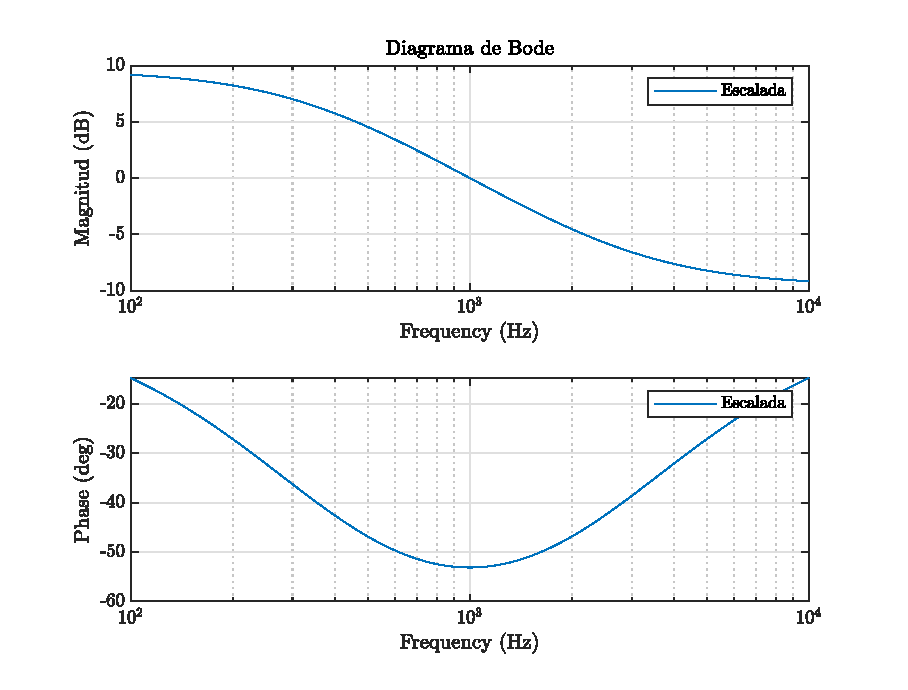
\includegraphics[width=8cm]{../imagenes/F12_bode_1er_orden_escalado.eps}
	\end{figure}
	\end{frame}
%%----------------------------------------------------------------------------------
%%----------------------------------------------------------------------------------
	\begin{frame}
		\frametitle{Implementación de integradores fraccionarios}
		\begin{block}{Ecuaciones de metodología bilineal polo y cero.}
			 \begin{equation}
	 \frac{G_{H}(s + 2 \pi f_{z})}{s + 2 \pi f_{p}} = \frac{As + k_{f}}{s + A k_{f}}
	 \label{ec:igualar_bilineal}
	 \end{equation}
	 de la ecuación (\ref{ec:igualar_bilineal}) se deducen las siguientes ecuaciones:
	 
	 \begin{equation}
		 G_{H} = A
		 \label{ec:bilineal_gh}
	 \end{equation}
	 
	 \begin{equation}
	 	f_{p} = \frac{A k_{f}}{2 \pi}
	 	\label{ec:bilineal_fp}
	 \end{equation}
	 
	 \begin{equation}
		f_{z} = \frac{k_{f}}{ 2A \pi}
		\label{ec:bilineal_fz}
	 \end{equation}
	 
	 \begin{equation}
	 G_{L} = \frac{1}{A}
	 \label{ec:bilineal_gl}
	 \end{equation}
		\end{block}
	\end{frame}
%%----------------------------------------------------------------------------------
%%----------------------------------------------------------------------------------
	\begin{frame}
		\frametitle{Implementación de integradores fraccionarios}
		\begin{minipage}[b]{0.45\textwidth}
			\begin{tiny}
			\begin{table}[!hbp]                                      
		\centering   
		\caption{Valores para configurar un filtro bilineal como integrador de orden fraccionario en el rango de ordenes de 0.1 a 0.95.}                            
		\label{tab:calculos_bilineal}                                        
			\begin{tabular}{ccccc}                        
			\hline                                              
			$\bm{\alpha}$ & $\bm{f_{p}}\,\,$ [kHz] & $\bm{f_{z}}\,\,$ [kHz] & $\bm{G_{L}}$ & $\bm{G_{H}}$ \\            
			\hline                                              
			0.10 & 0.818182 & 1.222222 & 1.222222 & 0.818182 \\  
			                                              
			0.15 & 0.739130 & 1.352941 & 1.352941 & 0.739130 \\  
			                                            
			0.20 & 0.666667 & 1.500000 & 1.500000 & 0.666667 \\  
			                                              
			0.25 & 0.600000 & 1.666667 & 1.666667 & 0.600000 \\  
			                                              
			0.30 & 0.538462 & 1.857143 & 1.857143 & 0.538462 \\  
			                                              
			0.35 & 0.481481 & 2.076923 & 2.076923 & 0.481481 \\  
			                                              
			0.40 & 0.428571 & 2.333333 & 2.333333 & 0.428571 \\  
			                                            
			0.45 & 0.379310 & 2.636364 & 2.636364 & 0.379310 \\  
			                                             
			0.50 & 0.333333 & 3.000000 & 3.000000 & 0.333333 \\  
			                                             
			0.55 & 0.290323 & 3.444444 & 3.444444 & 0.290323 \\  
			                                             
			0.60 & 0.250000 & 4.000000 & 4.000000 & 0.250000 \\  
			                                              
			0.65 & 0.212121 & 4.714286 & 4.714286 & 0.212121 \\  
			                                             
			0.70 & 0.176471 & 5.666667 & 5.666667 & 0.176471 \\  
			                                              
			0.75 & 0.142857 & 7.000000 & 7.000000 & 0.142857 \\  
			                                              
			0.80 & 0.111111 & 9.000000 & 9.000000 & 0.111111 \\  
			                                             
			0.85 & 0.081081 & 12.333333 & 12.333333 & 0.081081 \\
			                                              
			0.90 & 0.052632 & 19.000000 & 19.000000 & 0.052632 \\
			                                              
			0.95 & 0.025641 & 39.000000 & 39.000000 & 0.025641 \\
			\hline                                              
			\end{tabular}                                                                
	\end{table} 
			\end{tiny}
		\end{minipage} \hfill \begin{minipage}[b]{0.45\textwidth}
			\begin{figure}[hbtp]
		\caption{Gráfica de mérito, análisis de orden fraccionario dependiente de $n$ para implementación con CAM FilterBilinear.} 
		\label{fig:T11_Analisis_de_frecuencias_FilterBilinear}
		\centering
		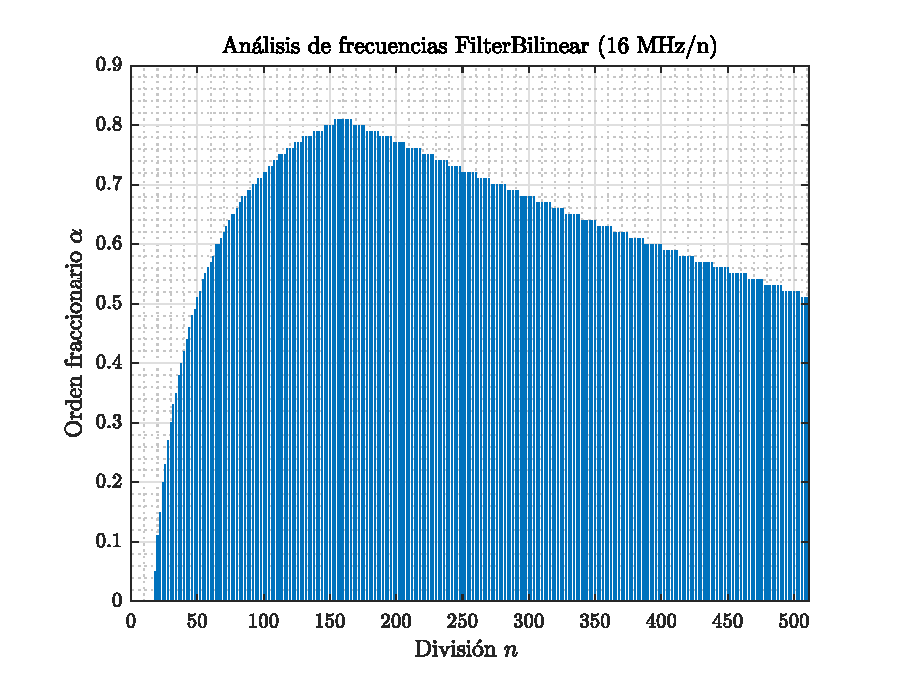
\includegraphics[width=6cm]{../imagenes/T11_Analisis_de_frecuencias_FilterBilinear.eps}
	\end{figure}
		\end{minipage}
	\end{frame}
%%----------------------------------------------------------------------------------
%%----------------------------------------------------------------------------------
	\begin{frame}
		\frametitle{Implementación de integradores fraccionarios}
		\begin{block}{Restricciones}
		\begin{footnotesize}
		\begin{table}[!hbp]                                      
		\centering   
		\caption{Rango de frecuencias absolutas dependiente de $F_{c}$ y el valor de $n$.}                            
		\label{tab:frecuencias_absolutas}                                        
			\begin{tabular}{cccc}                        
			\hline                                              
			$\bm{F_{c}}\,\,$ [kHz] & $\bm{n}$ & \textbf{min}$\bm{=F_{c} / 1000}\,\,$ [kHz] & \textbf{max}$\bm{=F_{c} /10}\,\,$ [kHz] \\                    
			\hline                                              
			16000.0000 & 1.0000 & 16.0000 & 1600.0000 \\
			                                     
			8000.0000 & 2.0000 & 8.0000 & 800.0000 \\   
			                                     
			4000.0000 & 4.0000 & 4.0000 & 400.0000 \\   
			
			$\vdots$ & $\vdots$ & $\vdots$ & $\vdots$ \\  
			 
			31.6206 & 506.0000 & 0.0316 & 3.1621 \\     
			                                    
			31.4961 & 508.0000 & 0.0315 & 3.1496 \\     
			                                    
			31.3725 & 510.0000 & 0.0314 & 3.1373 \\      
			\hline                                           
			\end{tabular}                                                                
	\end{table} 
		\end{footnotesize}
		\end{block}
	\end{frame}
%%----------------------------------------------------------------------------------
%%----------------------------------------------------------------------------------
	\begin{frame}
		\frametitle{Implementación de integradores fraccionarios}
		\begin{figure}[!ht] 
		\caption{Implementación de integrador de orden fraccionario utilizando la aproximación de primer orden.}
		\label{fig:G4_AD2_BilinearFilter_implementation}
		\centering
		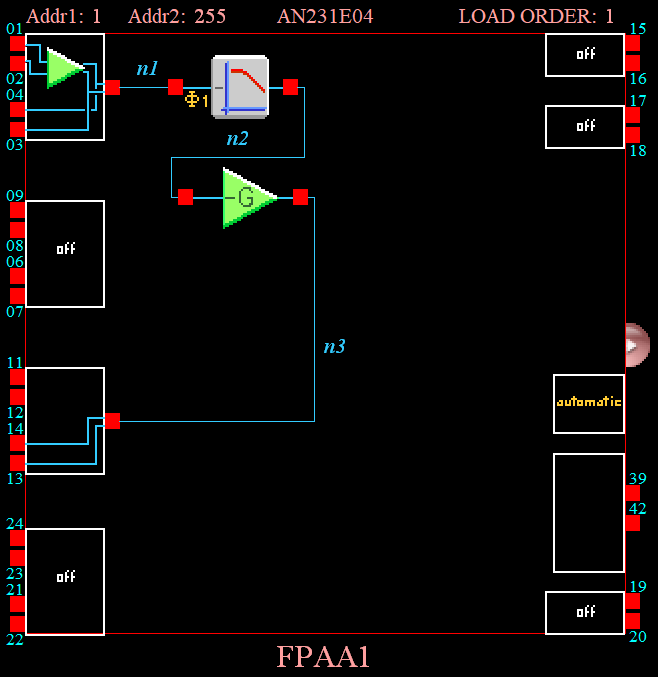
\includegraphics[width = 5.5cm]{../imagenes/G4_AD2_BilinearFilter_implementation.png}
	\end{figure}
	\end{frame}
%%----------------------------------------------------------------------------------
%%----------------------------------------------------------------------------------
	\begin{frame}
		\frametitle{Implementación de integradores fraccionarios}
		\begin{minipage}[t]{0.45\textwidth}
			\begin{figure}[!ht] 
		\caption{Resultados experimentales de respuesta en frecuencia con $\alpha = 0.5$.}
		\label{fig:M1_05}
		\centering
		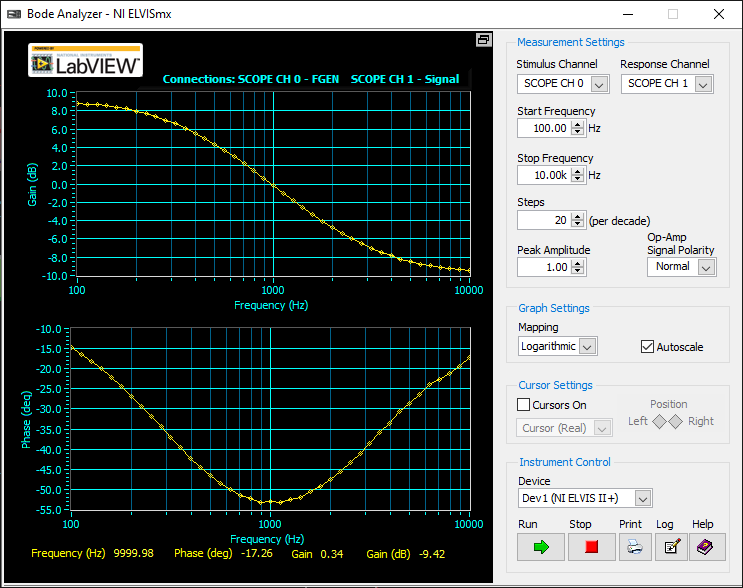
\includegraphics[width = 5cm]{../imagenes/M1_05.png}
	\end{figure}
		\end{minipage} \hfill \begin{minipage}[t]{0.45\textwidth}
			\begin{figure}[hbtp]
		\caption{Diagrama de bode de comparativo, respuesta teórica contra experimental,  $k_{f} = 2\pi 1000$ y  $\alpha = 0.5$.} 
		\label{fig:V13_comparacion_exp}
		\centering
		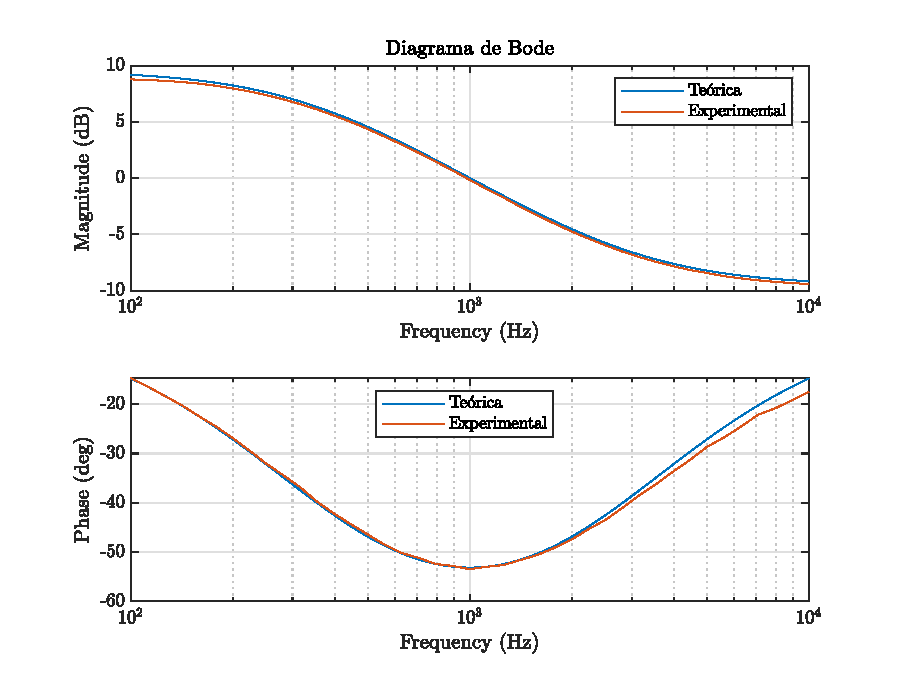
\includegraphics[width=6cm]{../imagenes/V13_comparacion_exp.eps}
	\end{figure}
		\end{minipage}
	\end{frame}
%%----------------------------------------------------------------------------------
%%----------------------------------------------------------------------------------
\begin{frame}
		\frametitle{Implementación de integradores fraccionarios}
		\begin{minipage}[t]{0.45\textwidth}
			\begin{figure}[!ht]
		\caption{Análisis transitorio de aproximación de primer orden.} 
		\label{fig:V14_analisis_transitorio}
		\centering
		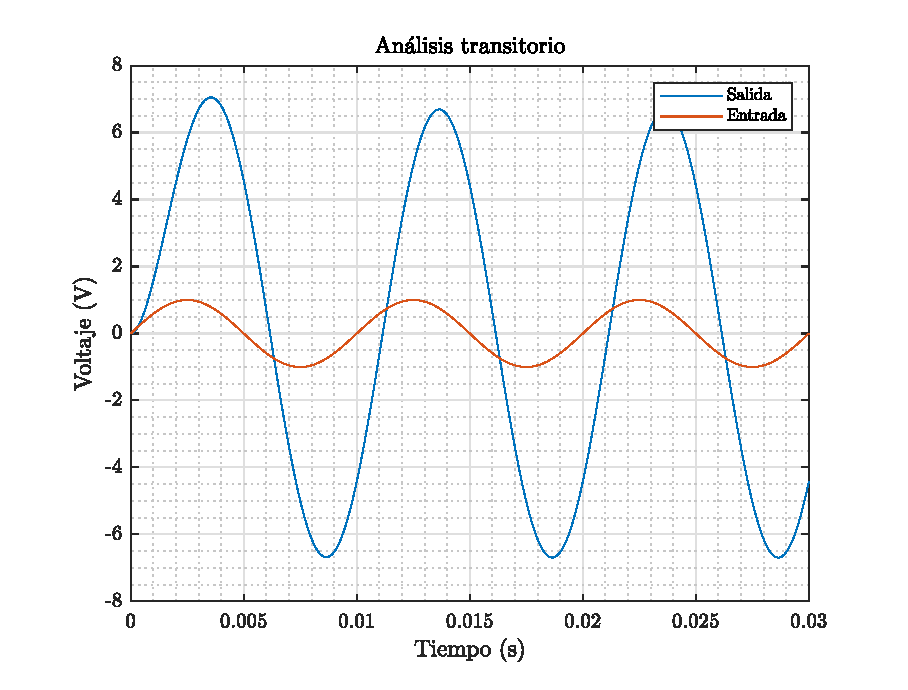
\includegraphics[width=5cm]{../imagenes/V14_analisis_transitorio.eps}
	\end{figure}
		\end{minipage} \hfill \begin{minipage}[t]{0.45\textwidth}
			\begin{figure}[!ht]
		\caption{Medición experimental de análisis transitorio.} 
		\label{fig:V15_transitorio_real}
		\centering
		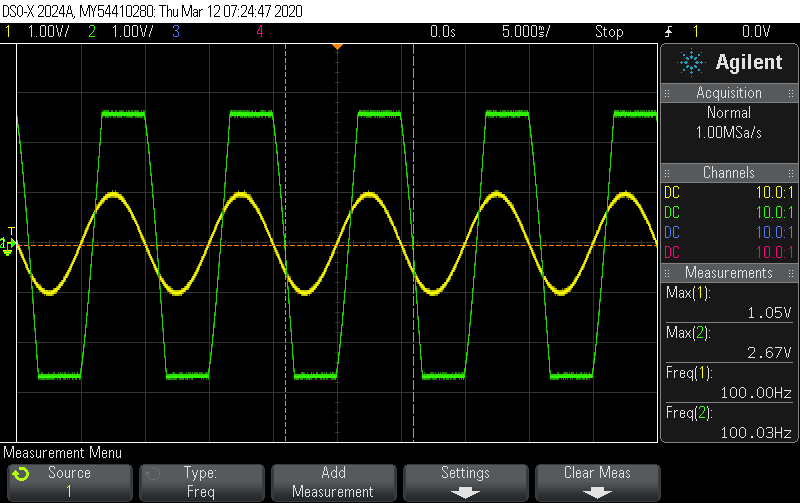
\includegraphics[width=5cm]{../imagenes/V15_transitorio_real.png}
	\end{figure}
		\end{minipage}
	\end{frame}
%%----------------------------------------------------------------------------------
%%----------------------------------------------------------------------------------	
	\begin{frame}
		\frametitle{Implementación de integradores fraccionarios}
		\begin{block}{Configuración bilineal pasabajas y pasaaltas}
		\textbf{CAM FilterBilinear}
			
	Pasabajas
	\begin{equation}
		\frac{V_{\mathrm{out}} (s)}{V_{\mathrm{in}}(s)} =  \pm \frac{2 \pi f_{0} G_{1}}{s + 2 \pi f_{0}}  
		\label{ec:CAM_bilinear_pasabajas}
	\end{equation}
	
	Pasaaltas
	\begin{equation}
	\frac{V_{\mathrm{out}} (s)}{V_{\mathrm{in}}(s)} =  - \frac{ G_{2} s}{s + 2 \pi f_{0}}
	\end{equation}
	
	Suma:
	\begin{equation}
		\frac{V_{\mathrm{out}} (s)}{V_{\mathrm{in}}(s)} = \frac{2 \pi f_{0} G_{1}}{s + 2 \pi f_{0}} + \frac{ G_{2} s}{s + 2 \pi f_{0}} = \frac{G_{2}s + G_{1}2 \pi f_{0}}{s + 2 \pi f_{0}}
		\label{ec:fun_trans_suma_filtros}
	\end{equation}
		\end{block}
	\end{frame}

%%----------------------------------------------------------------------------------
%%----------------------------------------------------------------------------------
	\begin{frame}
		\frametitle{Implementación de integradores fraccionarios}
		\begin{block}{Ecuaciones de metodología bilineal pabajas y pasaltas.}
			 \begin{equation}
		\frac{G_{2}s + G_{1}2 \pi f_{0}}{s + 2 \pi f_{0}} = \frac{As + k_{f}}{s + Ak_{f}}
		\label{ec:igualar_suma_filtros}
	\end{equation}
	de la ecuación (\ref{ec:igualar_suma_filtros}) se deducen las siguientes ecuaciones:
	
	\begin{equation}
		G_{1} = \frac{1}{A}
	\end{equation}	
	
	\begin{equation}
		G_{2} = A
	\end{equation}
	
	\begin{equation}
		f_{0} = \frac{A k_{f}}{2 \pi}
	\end{equation}
		\end{block}
	\end{frame}
%%----------------------------------------------------------------------------------
%%----------------------------------------------------------------------------------
	\begin{frame}
		\frametitle{Implementación de integradores fraccionarios}
		\begin{minipage}[b]{0.45\textwidth}
			\begin{tiny}
			\begin{table}[!hbp]                                      
		\centering   
		\caption{Valores para configurar implementación suma de pasabajas y pasaltas de ordenes de 0.1 a 0.95.}                            
		\label{tab:calculos_bilineal_suma}                                        
			\begin{tabular}{cccc}                        
			\hline                                              
			$\bm{\alpha}$ & $\bm{G_{1}}\,\,$ [LP] & $\bm{G_{2}}\,\,$ [HP] & $\bm{f_{0}}\,\,$ [kHz]  \\            
			\hline                                              
			0.10 & 1.222222 & 0.818182 & 0.818182 \\ 
			                                 
			0.15 & 1.352941 & 0.739130 & 0.739130 \\ 
			                                 
			0.20 & 1.500000 & 0.666667 & 0.666667 \\ 
			                                
			0.25 & 1.666667 & 0.600000 & 0.600000 \\ 
			                                  
			0.30 & 1.857143 & 0.538462 & 0.538462 \\ 
			                                  
			0.35 & 2.076923 & 0.481481 & 0.481481 \\ 
			                                  
			0.40 & 2.333333 & 0.428571 & 0.428571 \\ 
			                               
			0.45 & 2.636364 & 0.379310 & 0.379310 \\ 
			                                 
			0.50 & 3.000000 & 0.333333 & 0.333333 \\ 
			                                   
			0.55 & 3.444444 & 0.290323 & 0.290323 \\ 
			                                  
			0.60 & 4.000000 & 0.250000 & 0.250000 \\ 
			                                 
			0.65 & 4.714286 & 0.212121 & 0.212121 \\ 
			                                   
			0.70 & 5.666667 & 0.176471 & 0.176471 \\ 
			                                  
			0.75 & 7.000000 & 0.142857 & 0.142857 \\ 
			                                   
			0.80 & 9.000000 & 0.111111 & 0.111111 \\ 
			                                 
			0.85 & 12.333333 & 0.081081 & 0.081081 \\
			                                  
			0.90 & 19.000000 & 0.052632 & 0.052632 \\
			                                  
			0.95 & 39.000000 & 0.025641 & 0.025641 \\
			\hline                                              
			\end{tabular}                                                                
	\end{table}
			\end{tiny}
		\end{minipage} \hfill \begin{minipage}[b]{0.45\textwidth}
			\begin{figure}[hbtp]
		\caption{Gráfica de mérito, análisis de orden fraccionario dependiente de $n$ para implementación con suma de filtros.} 
		\label{fig:T12_Analisis_de_frecuencias_suma_de_filtros}
		\centering
		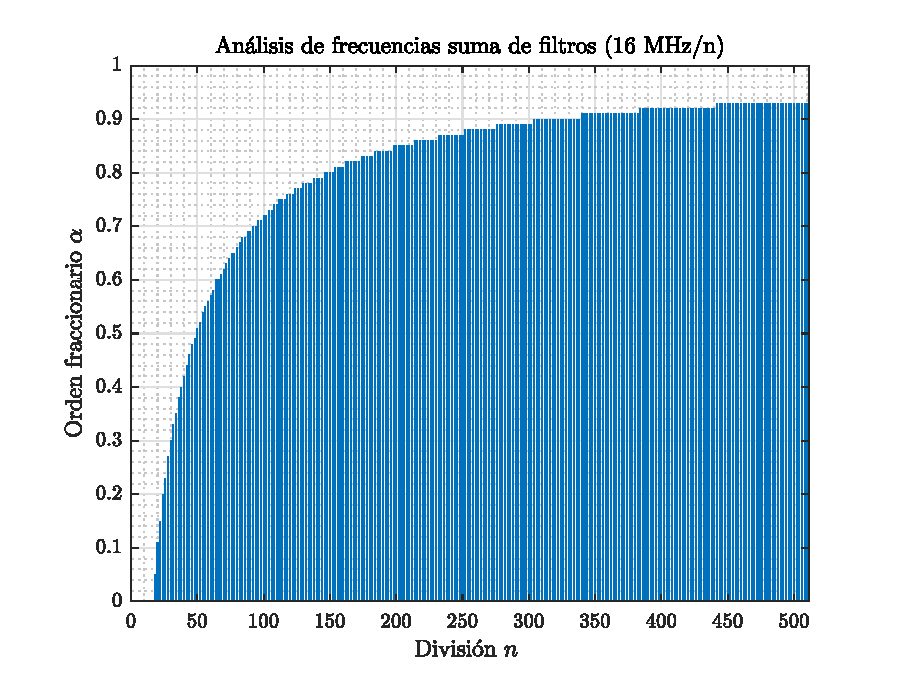
\includegraphics[width=6cm]{../imagenes/T12_Analisis_de_frecuencias_suma_de_filtros.eps}
	\end{figure}
		\end{minipage}
	\end{frame}
%%----------------------------------------------------------------------------------
%%----------------------------------------------------------------------------------
	\begin{frame}
		\frametitle{Implementación de integradores fraccionarios}
		\begin{figure}[!ht] 
		\caption{Implementación de integrador de orden fraccionario utilizando la aproximación de primer orden configuración suma de filtros.}
		\label{fig:V16_AD2_imple_suma_filtros}
		\centering
		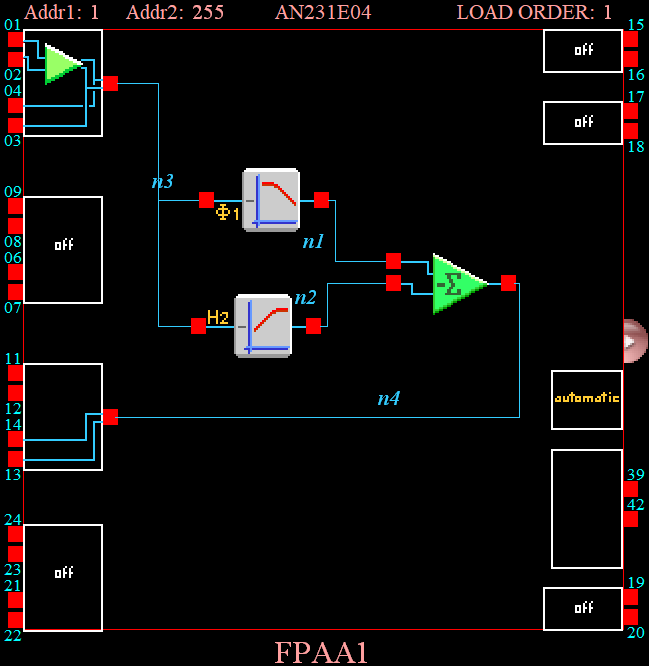
\includegraphics[width = 5.5cm]{../imagenes/V16_AD2_imple_suma_filtros.png}
	\end{figure}
	\end{frame}
%%----------------------------------------------------------------------------------
%%----------------------------------------------------------------------------------
	\begin{frame}
		\frametitle{Implementación de integradores fraccionarios}
		\begin{minipage}[t]{0.45\textwidth}
			\begin{figure}[!ht] 
		\caption{Resultados experimentales de respuesta en frecuencia con $\alpha = 0.5$ configuración de dos filtros y punto suma.}
		\label{fig:M2_05}
		\centering
		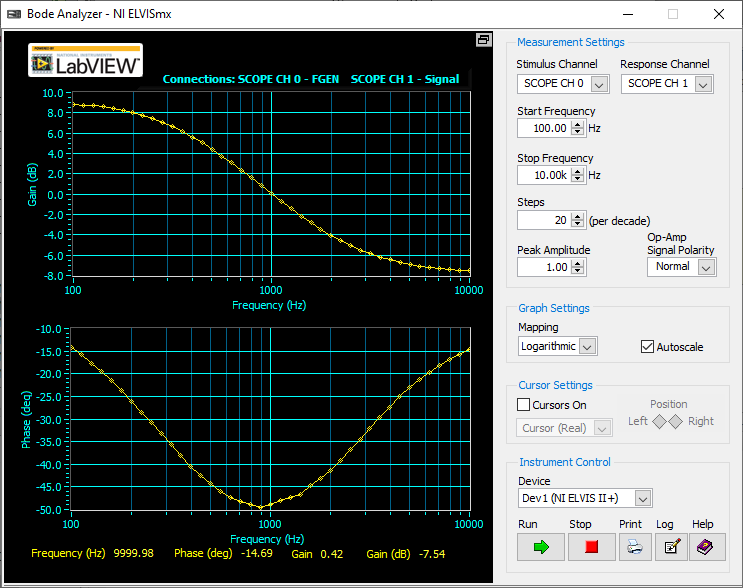
\includegraphics[width = 5cm]{../imagenes/M2_05.png}
	\end{figure}	
		\end{minipage} \hfill \begin{minipage}[t]{0.45\textwidth}
			\begin{figure}[!ht]
		\caption{Diagrama de bode de comparativo, respuesta teórica contra experimental configuración de dos filtros y punto suma,  $k_{f} = 2\pi 1000$ y  $\alpha = 0.5$.} 
		\label{fig:V15_bodes_comparativos_suma}
		\centering
		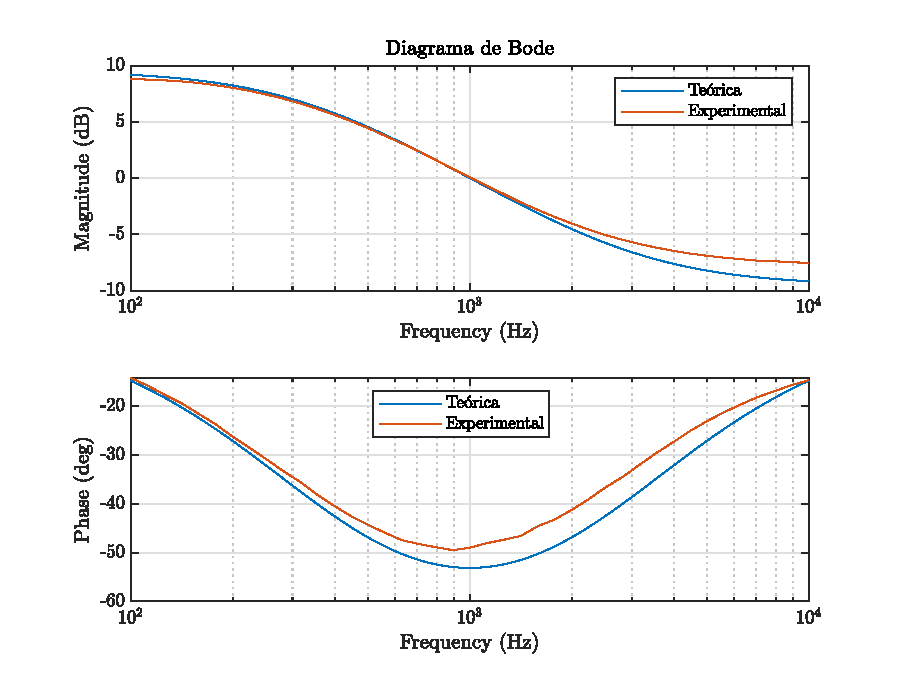
\includegraphics[width=6cm]{../imagenes/V15_bodes_comparativos_suma.eps}
	\end{figure}
		\end{minipage}
	\end{frame}







%%----------------------------------------------------------------------------------
%%----------------------------------------------------------------------------------	
	\begin{frame}
		\frametitle{Implementación de integradores fraccionarios}
		\begin{block}{Configuración bicuadratico polo y cero}
		\textbf{CAM FilterBiquad}
			\begin{equation}
		\frac{V_{\mathrm{out}} (s)}{V_{\mathrm{in}}(s)} = - \frac{G_{H} \left(  s^{2} + \cfrac{2 \pi f_{z}}{Q_{z}} s + 4 \pi^{2} f_{z}^{2} \right)}{s^{2} + \cfrac{2 \pi f_{p}}{Q_{p}}s + 4\pi^{2} f_{p}^{2} }
		\label{ec:CAM_biquad}
	\end{equation}
	
	\begin{equation}
		\genfrac{}{}{0pt}{0}{}{_{(c_{4})}} \frac{1}{s^{\alpha}} \approx \frac{(\alpha^{2} - 3\alpha + 2) s^{2} + (8 - 2 \alpha^{2})s + (\alpha^{2} + 3\alpha + 2) }{(\alpha^{2} + 3\alpha + 2) s^{2} + (8 - 2 \alpha^{2})s + (\alpha^{2} - 3\alpha + 2)}
		\label{ec:CFE_segundo_orden}
	\end{equation}
	
	\begin{equation}
		D = \frac{\alpha^{2} - 3 \alpha + 2}{\alpha^{2} + 3\alpha + 2} \qquad C = \frac{8 - 2 \alpha^{2}}{\alpha^{2} +  3 \alpha + 2}
	\end{equation}
	
	\begin{equation}
		\genfrac{}{}{0pt}{0}{}{_{(c_{4})}} \frac{1}{s^{\alpha}} \approx  \frac{D s^{2} + Cs + 1}{s^{2} + Cs + D} \quad \Longrightarrow \quad  N(s) = \frac{D s^{2} + C k_{f}s + k_{f}^{2}}{s^{2} + C k_{f}s + Dk_{f}^{2}}
		\label{ec:CFE_segundo_orden_2}
	\end{equation}
		\end{block}
	\end{frame}
%%----------------------------------------------------------------------------------
%%----------------------------------------------------------------------------------
	\begin{frame}
		\frametitle{Implementación de integradores fraccionarios}
		\begin{figure}[hbtp]
		\caption{Diagrama de bode de aproximación bicuadratico polo y cero para un integrador fraccionario con $k_{f} = 2\pi 1000$ y  $\alpha = 0.5$.} 
		\label{fig:V19_segundo_orden_esc}
		\centering
		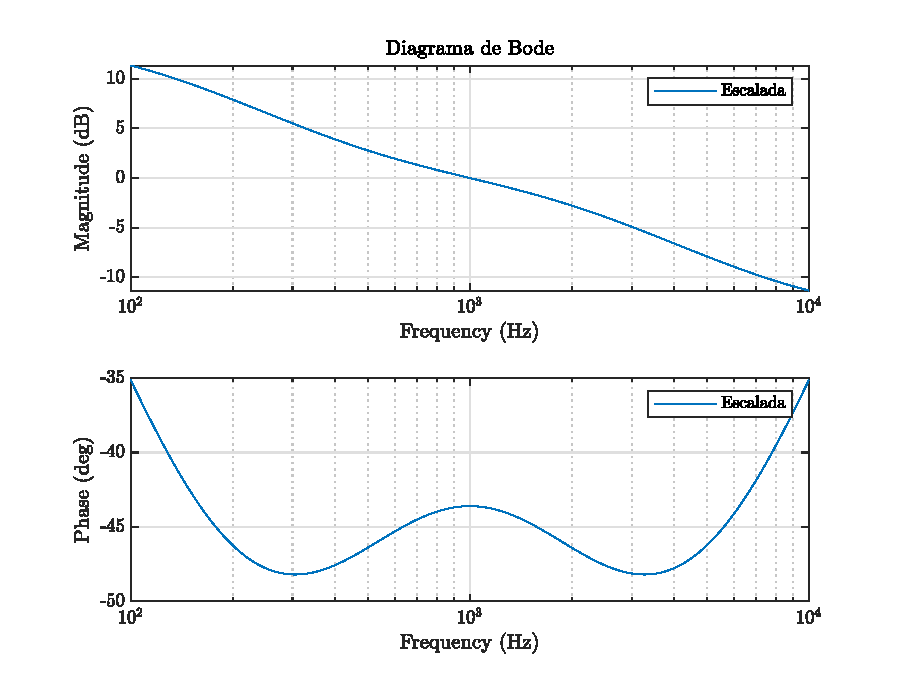
\includegraphics[width=8cm]{../imagenes/V19_segundo_orden_esc.eps}
	\end{figure}
	\end{frame}
%%----------------------------------------------------------------------------------
%%----------------------------------------------------------------------------------
	\begin{frame}
		\frametitle{Implementación de integradores fraccionarios}
		\begin{block}{Ecuaciones de metodología bicuadratico polo y cero 1.}
		\begin{equation}
		\frac{G_{H} \left(  s^{2} + \cfrac{2 \pi f_{z}}{Q_{z}} s + 4 \pi^{2} f_{z}^{2} \right)}{s^{2} + \cfrac{2 \pi f_{p}}{Q_{p}}s + 4\pi^{2} f_{p}^{2} } = \frac{D s^{2} + C k_{f}s + k_{f}^{2}}{s^{2} + C k_{f}s + Dk_{f}^{2}}
		\label{ec:igualdad_segundo_orden}
	\end{equation}
		
	\begin{equation}
		G_{H} = D  \qquad G_{L} = \frac{1}{D}
	\end{equation}
	
	\begin{equation}
		f_{z} = \frac{k_{f}}{2 \pi D^{\frac{1}{2}}} \qquad f_{p} = \frac{D^{\frac{1}{2}} k_{f}}{2 \pi}
	\end{equation}
	
	\begin{equation}
		Q_{z} = \frac{D^{\frac{1}{2}}}{C} \qquad Q_{p} = \frac{D^{\frac{1}{2}}}{C}	
	\end{equation}
	
		\end{block}
	\end{frame}
%%----------------------------------------------------------------------------------
%%----------------------------------------------------------------------------------
	\begin{frame}
		\frametitle{Implementación de integradores fraccionarios}
		\begin{block}{Ecuaciones de metodología bicuadratico polo y cero 2.}
		\begin{equation}
		\frac{G_{H} \left(  s^{2} + \cfrac{2 \pi f_{z}}{Q_{z}} s + 4 \pi^{2} f_{z}^{2} \right)}{s^{2} + \cfrac{2 \pi f_{p}}{Q_{p}}s + 4\pi^{2} f_{p}^{2} } = \frac{D s^{2} + C k_{f}s + k_{f}^{2}}{s^{2} + C k_{f}s + Dk_{f}^{2}}
	\end{equation}
		
		Elegir manualmente los factores de calidad $Q_{z}$ y $Q_{p}$ de modo que $\displaystyle{\gamma = \frac{Q_{z}}{Q_{p}}}$ y surjan las siguientes ecuaciones:
		
	\begin{equation}
		G_{H} = D  \qquad G_{L} = \frac{\gamma^{2}}{D}
	\end{equation}
	
	\begin{equation}
		f_{z} = \frac{C k_{f} Q_{z}}{D 2 \pi}	\qquad f_{p} = \frac{C k_{f} Q_{p}}{ 2 \pi}
	\end{equation}
	
		\end{block}
	\end{frame}
%%----------------------------------------------------------------------------------
%%----------------------------------------------------------------------------------
	\begin{frame}
		\frametitle{Implementación de integradores fraccionarios}
		\begin{minipage}[b]{0.45\textwidth}
			\begin{tiny}
			\begin{table}[!hbp]                                      
		\centering   
		\caption{Valores para configurar implementación de segundo orden FilterBiquad de ordenes de 0.1 a 0.95.}                            
		\label{tab:calculos_biquad}                                        
			\begin{tabular}{cccccc}                        
			\hline                                              
			$\bm{\alpha}$ & $\bm{G_{H}}\,\,$  & $\bm{G_{L}}\,\,$  & $\bm{f_{z}}\,\,$ [kHz] & $\bm{f_{p}}\,\,$ [kHz] & $\bm{Q_{z} = Q_{p}}\,\,$  \\            
			\hline                                              
			0.10 & 0.740260 & 1.350877 & 1.162272 & 0.860383 & 0.249058 \\   
		                                                          
			0.15 & 0.635996 & 1.572337 & 1.253929 & 0.797494 & 0.247870 \\   
		                                                        
			0.20 & 0.545455 & 1.833333 & 1.354006 & 0.738549 & 0.246183 \\   
	                                                          
			0.25 & 0.466667 & 2.142857 & 1.463850 & 0.683130 & 0.243975 \\   
		                                                        
			0.30 & 0.397993 & 2.512605 & 1.585120 & 0.630867 & 0.241214 \\   
		                                                          
			0.35 & 0.338061 & 2.958042 & 1.719896 & 0.581431 & 0.237858 \\   
			                                                        
			0.40 & 0.285714 & 3.500000 & 1.870829 & 0.534522 & 0.233854 \\   
		                                                          
			0.45 & 0.239972 & 4.167155 & 2.041361 & 0.489869 & 0.229132 \\   
			                                                          
			0.50 & 0.200000 & 5.000000 & 2.236068 & 0.447214 & 0.223607 \\   
		                                                         
			0.55 & 0.165085 & 6.057471 & 2.461193 & 0.406307 & 0.217164 \\   
			                                                         
			0.60 & 0.134615 & 7.428571 & 2.725541 & 0.366900 & 0.209657 \\   
		                                                         
			0.65 & 0.108062 & 9.253968 & 3.042034 & 0.328727 & 0.200889 \\   
		                                                          
			0.70 & 0.084967 & 11.769231 & 3.430631 & 0.291492 & 0.190591 \\  
		                                                         
			0.75 & 0.064935 & 15.400000 & 3.924283 & 0.254824 & 0.178377 \\  
			                                                          
			0.80 & 0.047619 & 21.000000 & 4.582576 & 0.218218 & 0.163663 \\  
		                                                         
			0.85 & 0.032717 & 30.565217 & 5.528582 & 0.180878 & 0.145489 \\  
			                                                         
			0.90 & 0.019964 & 50.090909 & 7.077493 & 0.141293 & 0.122026 \\  
			                                                           
			0.95 & 0.009126 & 109.571429 & 10.467637 & 0.095533 & 0.088709 \\
			\hline                                              
			\end{tabular}                                                                
	\end{table}
			\end{tiny}
		\end{minipage} \hfill \begin{minipage}[b]{0.45\textwidth}
			\begin{figure}[hbtp]
		\caption{Gráfica de mérito, análisis de orden fraccionario dependiente de $n$ para implementación con CAM FilterBiquad teórica INCORRECTA.} 
		\label{fig:W4_analisis_frecuencias_biquad}
		\centering
		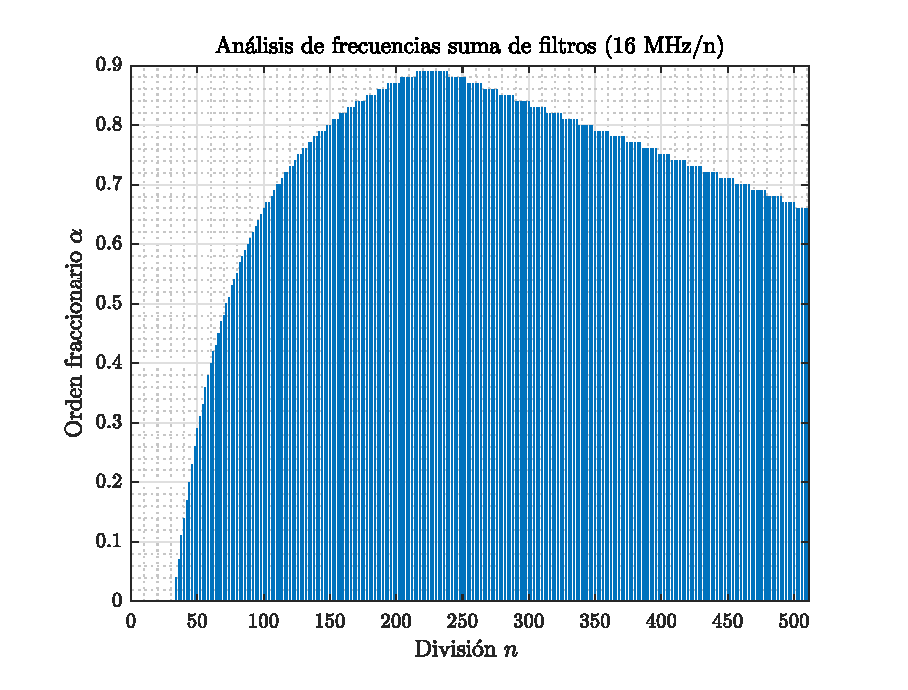
\includegraphics[width=6cm]{../imagenes/W4_analisis_frecuencias_biquad.eps}
	\end{figure}
		\end{minipage}
	\end{frame}
%%----------------------------------------------------------------------------------
%%----------------------------------------------------------------------------------
	\begin{frame}
		\frametitle{Implementación de integradores fraccionarios}
		\begin{figure}[!ht] 
		\caption{Implementación de integrador de orden fraccionario utilizando la aproximación de segundo orden.}
		\label{fig:W3_AD2_biquad}
		\centering
		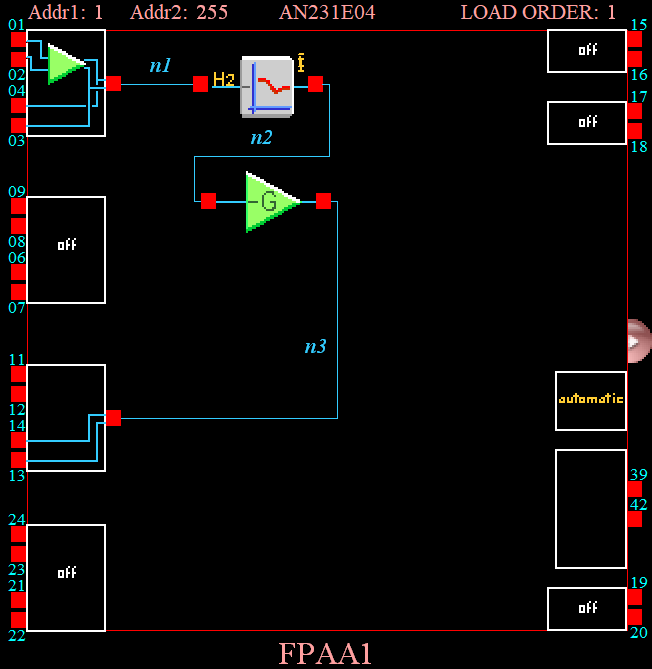
\includegraphics[width = 5.5cm]{../imagenes/W3_AD2_biquad}
	\end{figure}
	\end{frame}
%%----------------------------------------------------------------------------------
%%----------------------------------------------------------------------------------
	\begin{frame}
		\frametitle{Implementación de integradores fraccionarios}
		\begin{minipage}[t]{0.45\textwidth}
			\begin{figure}[!ht] 
		\caption{Resultados experimentales de respuesta en frecuencia con $\alpha = 0.5$.}
		\label{fig:W1_impl_seg_ord}
		\centering
		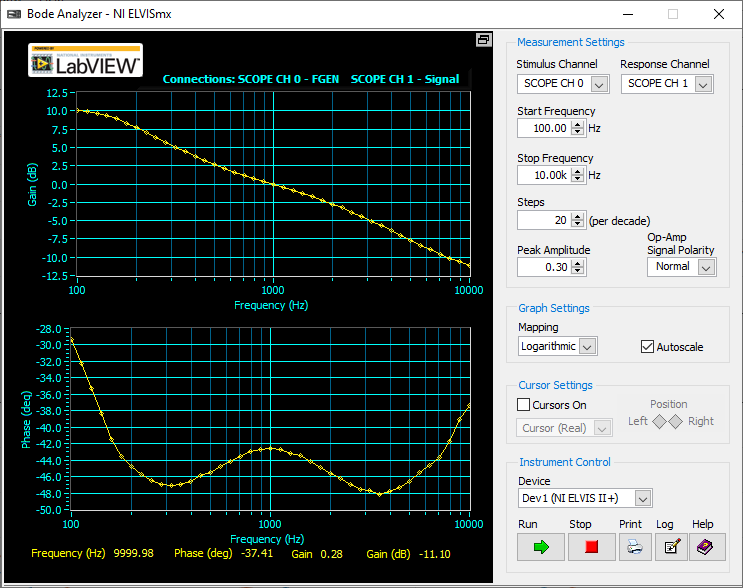
\includegraphics[width = 5cm]{../imagenes/W1_impl_seg_ord.png}
	\end{figure}
		\end{minipage} \hfill \begin{minipage}[t]{0.45\textwidth}
			\begin{figure}[!ht]
		\caption{Diagrama de bode de comparativo, respuesta teórica contra experimental,  $k_{f} = 2\pi 1000$ y  $\alpha = 0.5$.} 
		\label{fig:W2_seg_ord_teoria_exp}
		\centering
		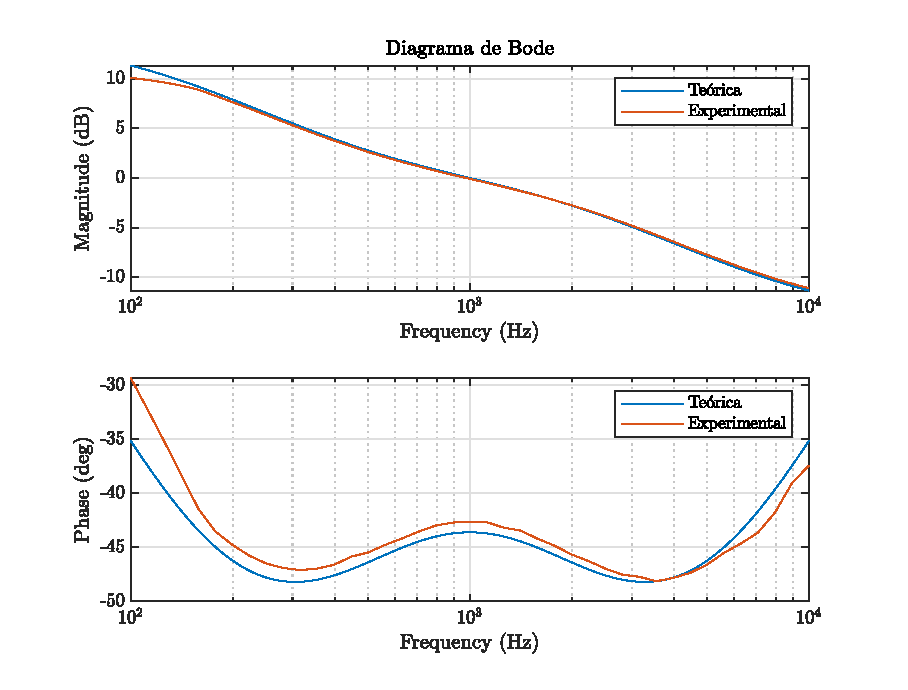
\includegraphics[width=6cm]{../imagenes/W2_seg_ord_teoria_exp.eps}
	\end{figure}
		\end{minipage}
	\end{frame}
	%%----------------------------------------------------------------------------------
%%----------------------------------------------------------------------------------
	\begin{frame}
		\frametitle{Implementación de integradores fraccionarios}
		\begin{block}{Resumen}
		\begin{scriptsize}
			\begin{table}[!ht]
	  \centering
	  \caption{Resumen de configuraciones para aproximación de integradores fraccionarios utilizando la CFE.}
	  \label{tab:resumen_config}
	  \begin{tabular}{>{\centering\arraybackslash}m{2cm} >{\centering\arraybackslash}m{1cm} >{\centering\arraybackslash}m{3cm} >{\centering\arraybackslash}m{3cm}}
	    \hline
	    \textbf{Configuración} & \textbf{Rango} $\bm{\alpha}$ & \textbf{Ventajas}  & \textbf{Desventajas}\\ 
	    \hline
	      Bilineal polo y cero
	    &
	     $[0.01, 0.81]$
	    & 
	      \begin{itemize}[leftmargin=0cm,noitemsep]
	      \begin{scriptsize}
			\item[] Consume pocos recursos.
			\item[] Facilidad de implementación.
			\item[] Proceso de diseño sencillo.
	      \end{scriptsize}
	      \end{itemize}
	     & 
	      \begin{itemize}[leftmargin=0cm,noitemsep]
	      \begin{scriptsize}
			\item[] Mayor error para $\alpha$ grande.
			\item[] Menor rango.
	      \end{scriptsize}
	      \end{itemize}
	    \\ %-------------------------------------------------------
	      Bilineal LP y HP
	    &
	      $[0.01, 0.93]$
	    & 
	      \begin{itemize}[leftmargin=0cm,noitemsep]
	      \begin{scriptsize}
			\item[] Mayor rango.
			\item[] Ajuste de ganancia flexible.
			\item[] Proceso de diseño sencillo.
	      \end{scriptsize}
	      \end{itemize}
	     & 
	      \begin{itemize}[leftmargin=0cm,noitemsep]
	      \begin{scriptsize}
			\item[] Consume más recursos.
			\item[] Mayor error que configuración polo y cero.
	      \end{scriptsize}
	      \end{itemize}
	    \\ %-------------------------------------------------------
	     	Bicuadrático
	    &
	      $[0.01, 0.6]$
	    & 
	      \begin{itemize}[leftmargin=0cm,noitemsep]
	      \begin{scriptsize}
			\item[] Menor error.
			\item[] Oportunidad de nuevos esquemas de diseño.
	      \end{scriptsize}
	      \end{itemize}
	     & 
	      \begin{itemize}[leftmargin=0cm,noitemsep]
	      \begin{scriptsize}
			\item[] Proceso de diseño complejo.
			\item[] Menor rango.
	      \end{scriptsize}
	      \end{itemize}
	    \\ %-------------------------------------------------------
	    \hline
	  \end{tabular}
	\end{table}
		\end{scriptsize}
		\end{block}
	\end{frame}
%%----------------------------------------------------------------------------------
%%----------------------------------------------------------------------------------
	\section{Oscilador caótico}
	\begin{frame}
		\frametitle{Oscilador caótico}
		\begin{block}{Oscilador caótico fraccionario basado en funciones no lineales saturadas (SNLF)}
			\begin{equation}
		 \begin{array}{lcl}
		_{0}D_{t}^{\alpha}x & = & y \\
		_{0}D_{t}^{\alpha}y  & = & z\\
		_{0}D_{t}^{\alpha}z  & = & -ax - by -cz + hf(x)
		\end{array}
		\label{ec:frac_osc_imp}
	\end{equation}
	donde  $a, b, c$ y $h$ son coeficientes reales positivas. $f(x)$ es una función lineal a trozos conocida como deestabilizadora o función saturada.
		\end{block}
	\end{frame}
%%----------------------------------------------------------------------------------
%%----------------------------------------------------------------------------------
	\begin{frame}
		\frametitle{Oscilador caótico}
		\begin{block}{Función deestabilizadora}
			 \begin{equation}
		f(x) = \left\{ \begin{array}{lcl}
		k & \mathrm{si} & x > \beta \\
		sx & \mathrm{si} & - \beta \leq x \leq \beta  \\
		-k & \mathrm{si} & x < -\beta
		\end{array}
		\right.
		\label{ec:saturacion}
	\end{equation}
	donde el parámetro $k$ representa la saturación del sistema, $\beta$ es el punto de quiebre en la función y $s$ es la pendiente entre tramos.
		\begin{figure}[!ht]
		\caption{Función no lineal saturada de dos enrollamientos.} 
		\label{fig:Z1_saturacion}
		\centering
		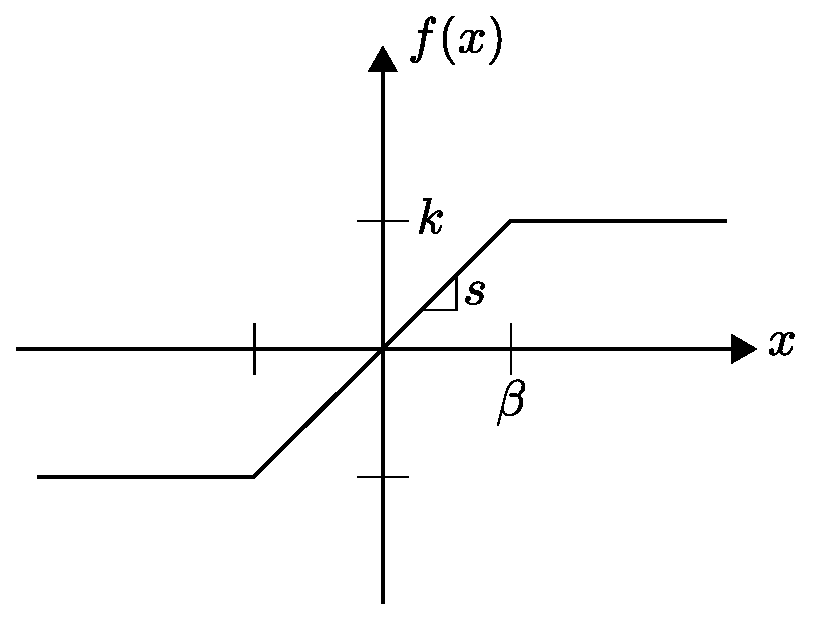
\includegraphics[width=4cm]{../imagenes/Z1_saturacion.eps}
	\end{figure}	
		\end{block}
	\end{frame}
%%----------------------------------------------------------------------------------
%%----------------------------------------------------------------------------------
	\begin{frame}
		\frametitle{Oscilador caótico}
		\begin{block}{ }
		\begin{figure}[!ht]
		\caption{Solución de sistema de orden fraccionario.}
		\label{fig:Z2_bloques}
		\centering
		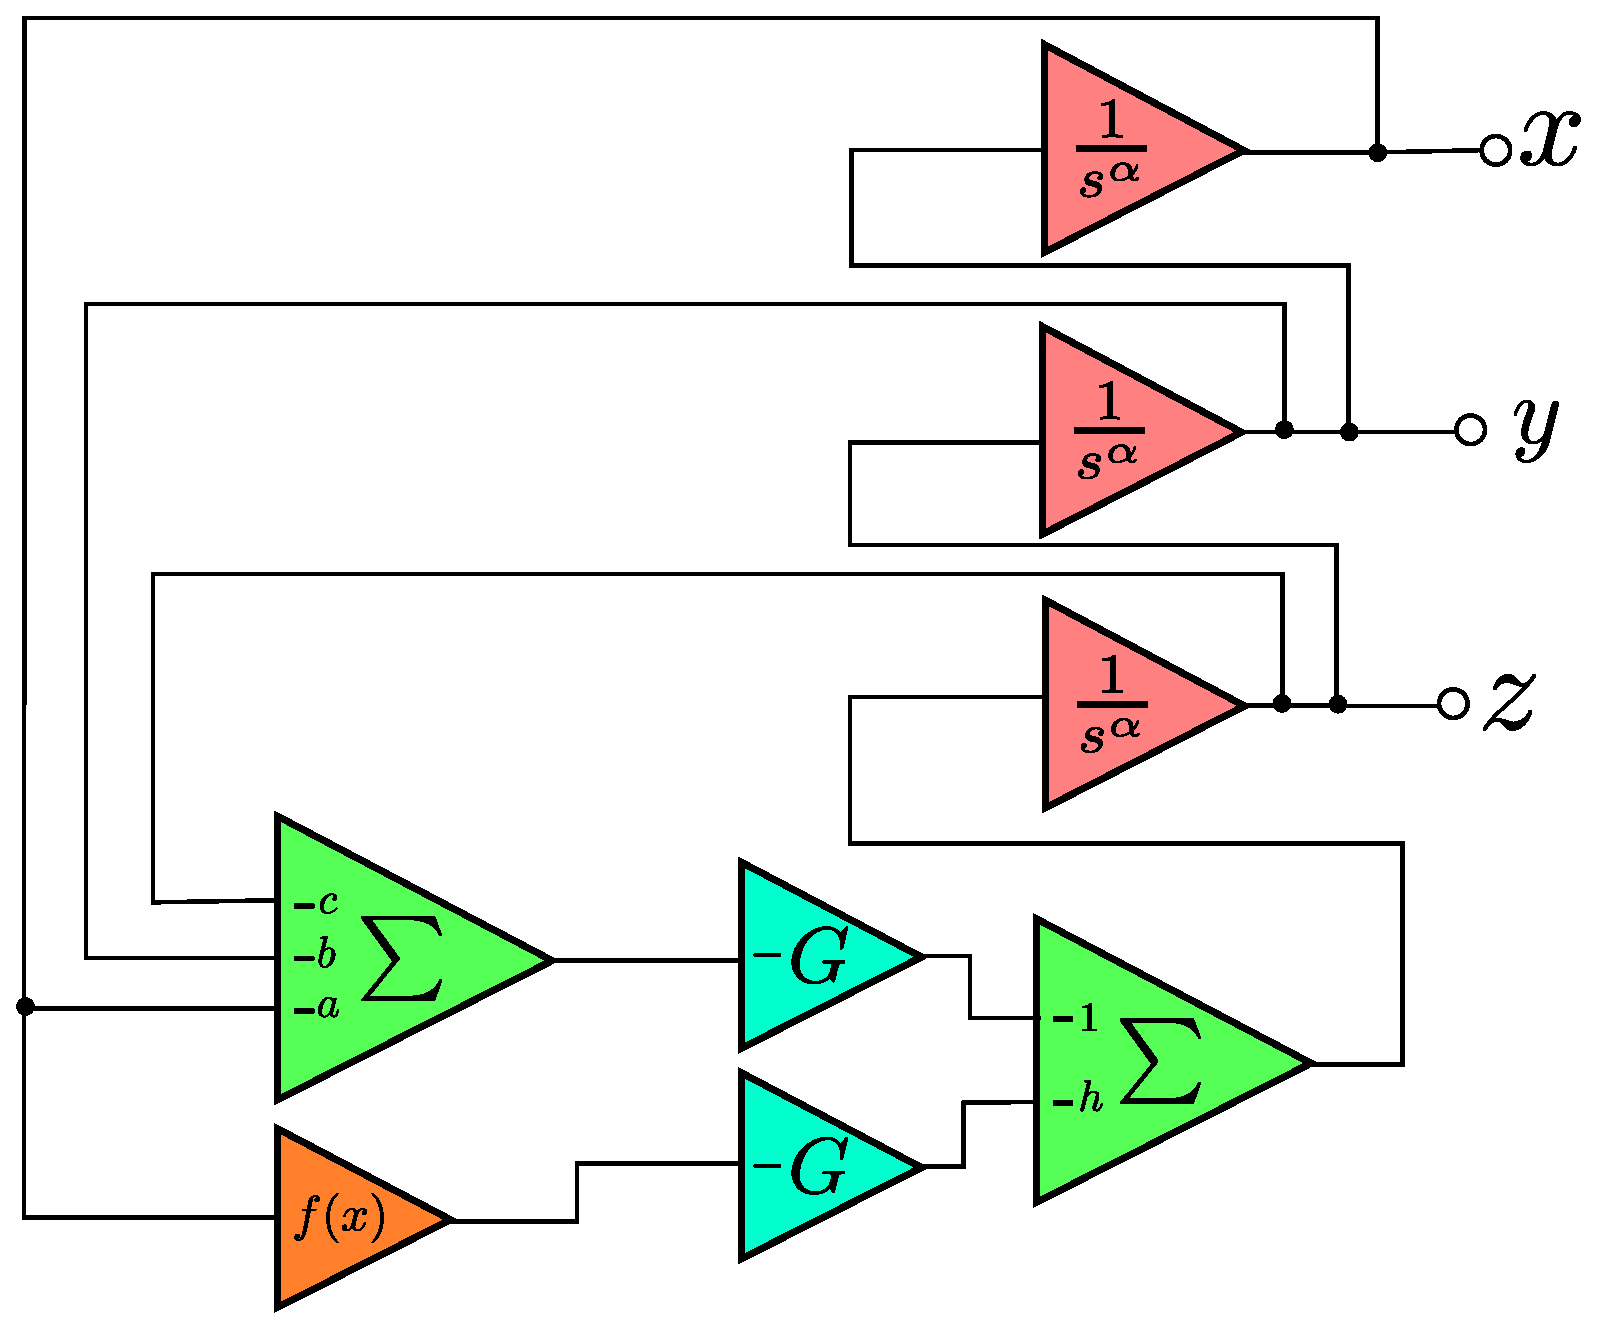
\includegraphics[width=7cm]{../imagenes/Z2_bloques.eps}
	\end{figure}
		\end{block}
	\end{frame}
%%----------------------------------------------------------------------------------
%%----------------------------------------------------------------------------------
	\begin{frame}
		\frametitle{Oscilador caótico}
		\begin{block}{Implementación de oscilador caótico}
		\begin{itemize}
			\item Utilizando filtro bilineal polo y cero.
			\item $\alpha = 0.8$.
			\item Dos enrollamientos.
		\end{itemize}
		\end{block}
	\end{frame}	
%%----------------------------------------------------------------------------------
%%----------------------------------------------------------------------------------
	\begin{frame}
		\frametitle{Oscilador caótico}
		\begin{figure}[!ht]
		\caption{Implementación en AD2 configuración bilineal polo y cero.} 
		\label{fig:Y1_implementacion}
		\centering
		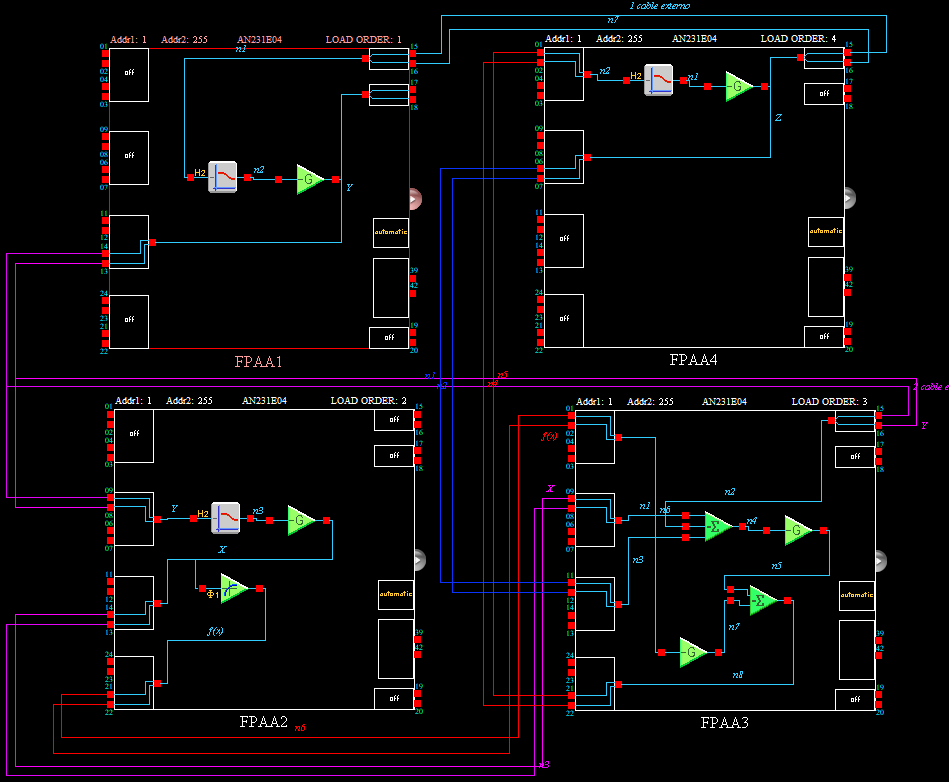
\includegraphics[width=8cm]{../imagenes/Y1_implementacion.png}
	\end{figure}
	\end{frame}		
%%----------------------------------------------------------------------------------
%%----------------------------------------------------------------------------------
	\begin{frame}
		\frametitle{Oscilador caótico}
		\begin{figure}[!ht]
				
		\textbf{Topología de filtro bilineal}
	\caption{Vistas de plano fase del comportamiento del oscilador caótico con $\alpha = 0.8$ y dos enrollamientos.}
	\label{fig:fase_imp_osc}
	  \begin{subfigure}[b]{0.3\textwidth}
	    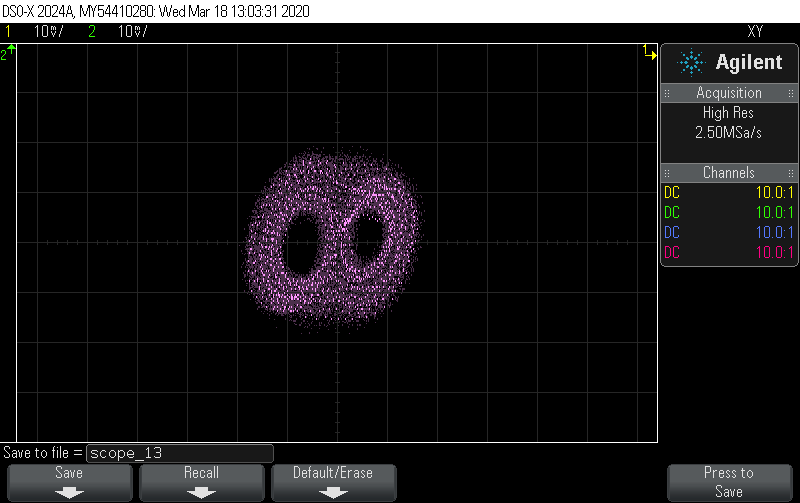
\includegraphics[trim={6cm 2cm 9cm 2cm},clip,width=\textwidth]{../imagenes/Y2_X_vs_Y.png}
	    \caption{$x$ vs $y$}
	    \label{Y2_X_vs_Y}
	  \end{subfigure}
	  \hfill
	  \begin{subfigure}[b]{0.3\textwidth}
	    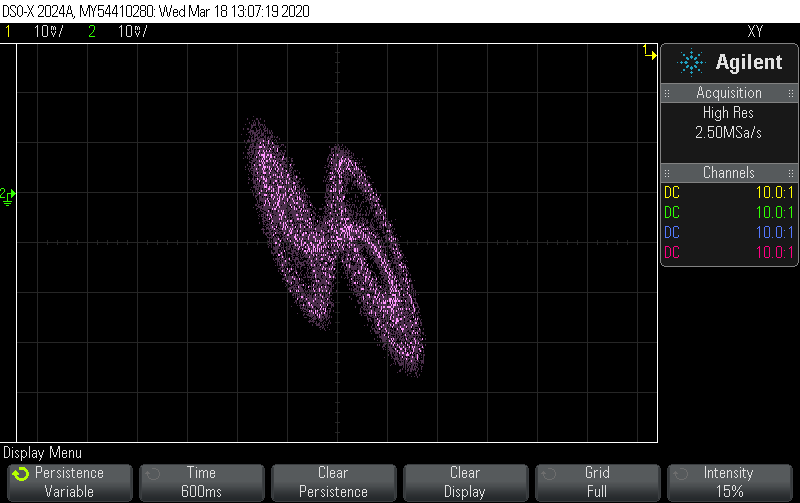
\includegraphics[trim={6cm 2cm 9cm 2cm},clip,width=\textwidth]{../imagenes/Y4_X_vs_Z.png}
	    \caption{$x$ vs $z$}
	    \label{fig:Y4_X_vs_Z}
	  \end{subfigure}
	  \hfill
	  \begin{subfigure}[b]{0.3\textwidth}
	    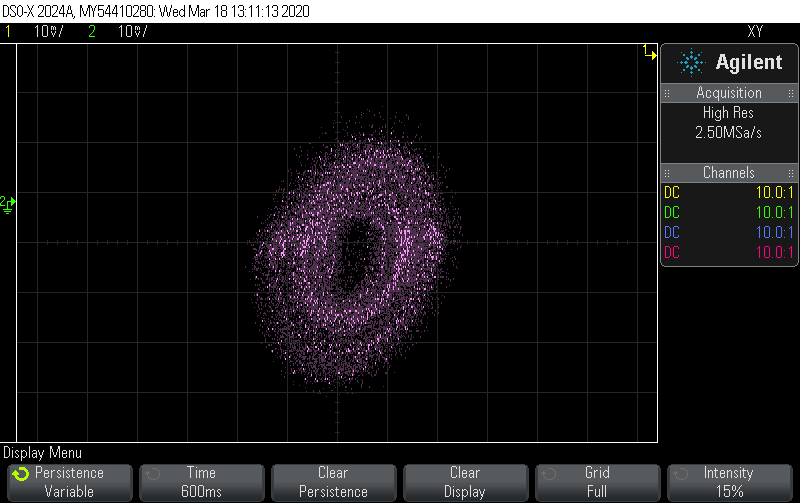
\includegraphics[trim={6cm 2cm 9cm 2cm},clip,width=\textwidth]{../imagenes/Y6_Y_vs_Z.png}
	    \caption{$y$ vs $z$}
	    \label{Y6_Y_vs_Z}
	  \end{subfigure}
	\end{figure}
	\end{frame}	
%%----------------------------------------------------------------------------------
%%----------------------------------------------------------------------------------
	\begin{frame}
		\frametitle{Oscilador caótico}
		\begin{figure}[!ht]
		\textbf{Topología de filtro bilineal}
	\caption{Respuesta en el dominio temporal de oscilador caótico con $\alpha = 0.8$ y dos enrollamientos.}
	\label{fig:temporal_imp}
	  \begin{subfigure}[b]{0.3\textwidth}
	    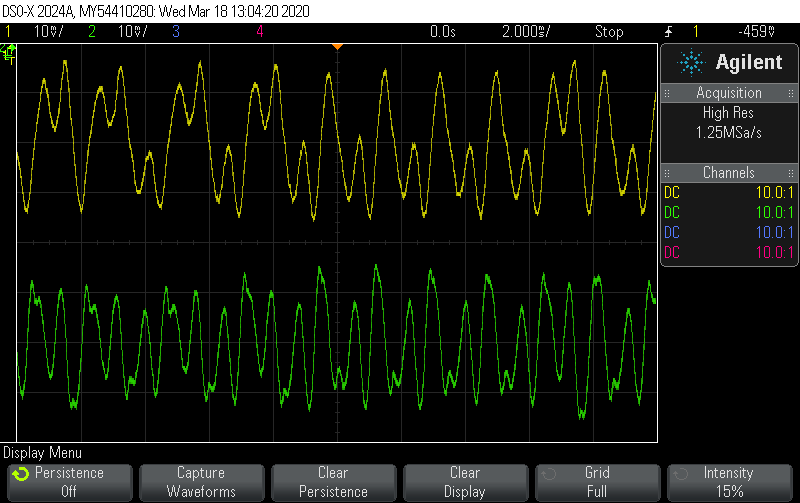
\includegraphics[trim={6cm 2cm 9cm 2cm},clip,width=\textwidth]{../imagenes/Y3_X_vs_Y_signal.png}
	    \caption{$x$,$y$ respecto al tiempo.}
	    \label{fig:Y3_X_vs_Y_signal}
	  \end{subfigure}
	  \hfill
	  \begin{subfigure}[b]{0.3\textwidth}
	    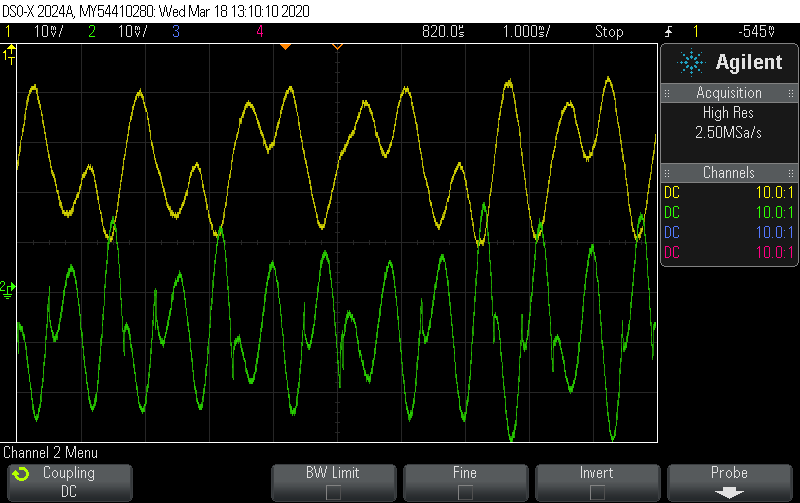
\includegraphics[trim={6cm 2cm 9cm 2cm},clip,width=\textwidth]{../imagenes/Y5_X_vs_Z_signal.png}
	    \caption{$x$,$z$ respecto al tiempo.}
	    \label{fig:Y5_X_vs_Z_signal}
	  \end{subfigure}
	  \hfill
	  \begin{subfigure}[b]{0.3\textwidth}
	    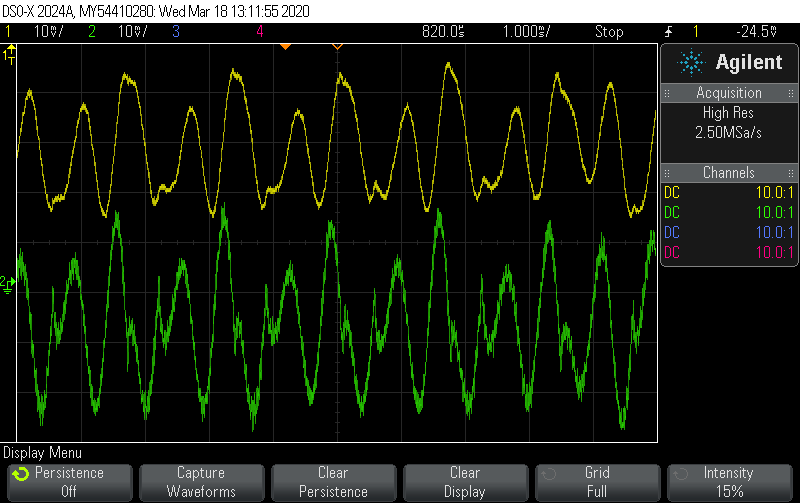
\includegraphics[trim={6cm 2cm 9cm 2cm},clip,width=\textwidth]{../imagenes/Y7_Y_vs_Z_signal.png}
	    \caption{$y$,$z$ respecto al tiempo.}
	    \label{fig:Y7_Y_vs_Z_signal}
	  \end{subfigure}
	\end{figure}	
	\end{frame}
%%----------------------------------------------------------------------------------
%%----------------------------------------------------------------------------------
	
	
	
	
		\begin{frame}
		\frametitle{Oscilador caótico}
		\begin{block}{Implementación de oscilador caótico}
		\begin{itemize}
			\item Utilizando filtro bilineal en suma de filtros pasabajas y pasaaltas.
			\item $\alpha = 0.8$.
			\item Dos enrollamientos.
		\end{itemize}
		\end{block}
	\end{frame}	
	
	
	
	
	
	
	
	\begin{frame}
		\frametitle{Oscilador caótico}
		\begin{figure}[!ht]
		\caption{Implementación en AD2 configuración bilineal pasabajas y pasaltas.} 
		\label{fig:Y1p_implementacion}
		\centering
		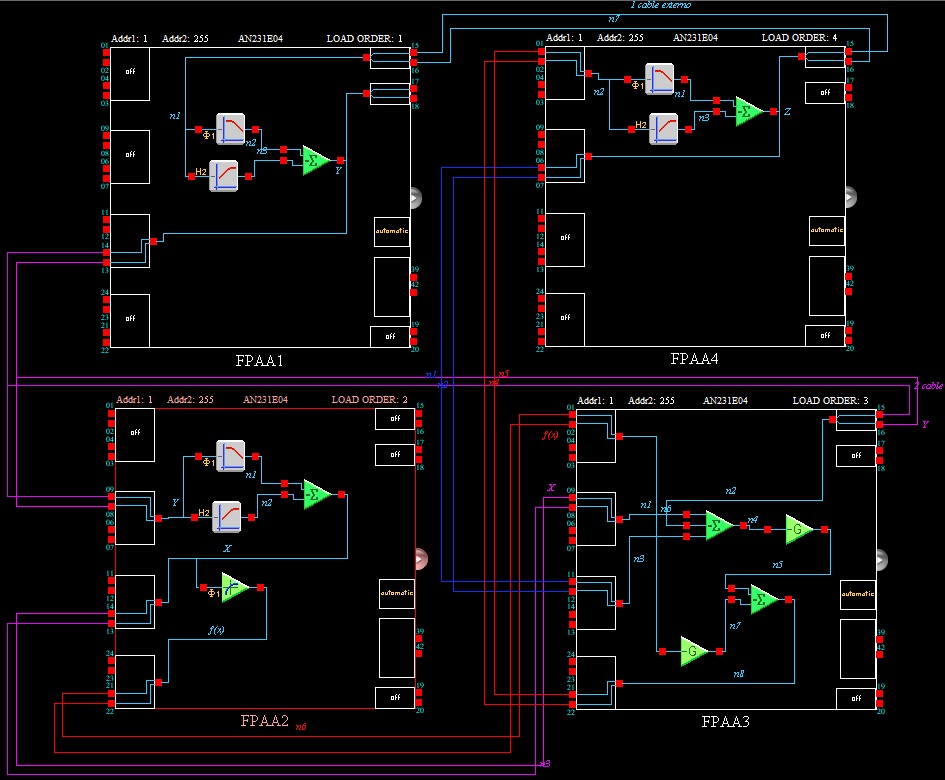
\includegraphics[width=8cm]{../imagenes/Y1p_implementacion.png}
	\end{figure}
	\end{frame}		
%%----------------------------------------------------------------------------------
%%----------------------------------------------------------------------------------
	
	
	
	
	\begin{frame}
		\frametitle{Oscilador caótico}
		\begin{figure}[!ht]
		\textbf{Topología de suma de filtros}
	\caption{Vistas de plano fase del comportamiento del oscilador caótico con $\alpha = 0.8$ y dos enrollamientos.}
	\label{fig:fase_imp_osc}
	  \begin{subfigure}[b]{0.3\textwidth}
	    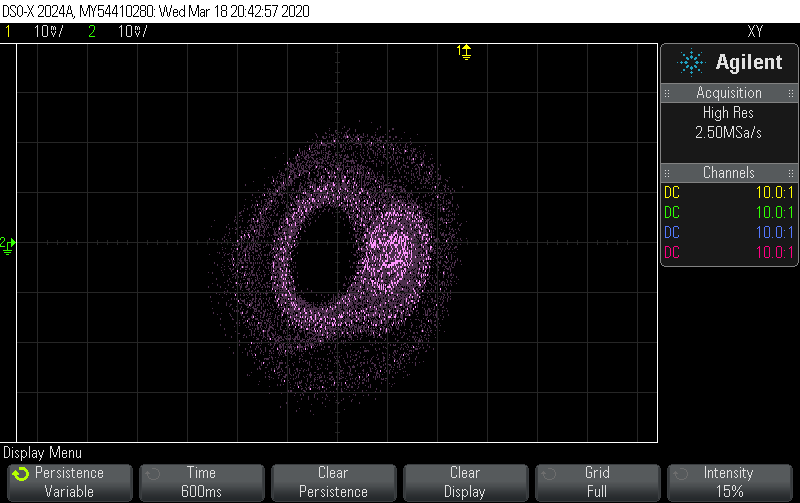
\includegraphics[trim={6cm 2cm 9cm 2cm},clip,width=\textwidth]{../imagenes/Y2p_X_vs_Y.png}
	    \caption{$x$ vs $y$}
	    \label{Y2p_X_vs_Y}
	  \end{subfigure}
	  \hfill
	  \begin{subfigure}[b]{0.3\textwidth}
	    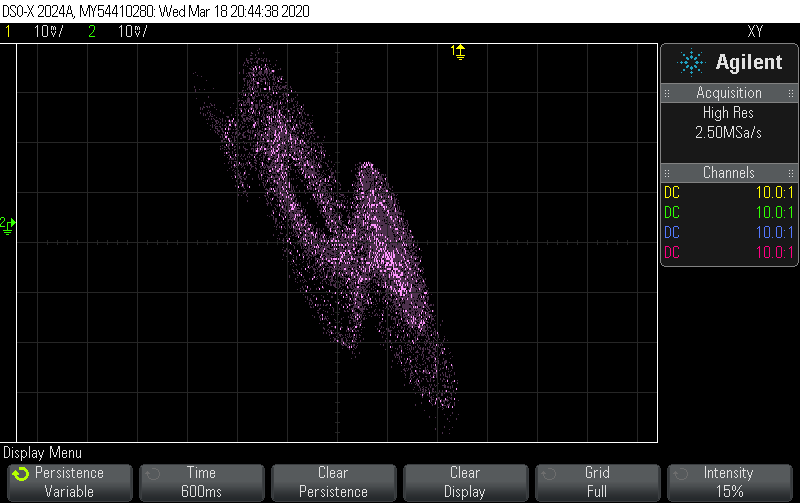
\includegraphics[trim={6cm 2cm 9cm 2cm},clip,width=\textwidth]{../imagenes/Y4p_X_vs_Z.png}
	    \caption{$x$ vs $z$}
	    \label{fig:Y4p_X_vs_Z}
	  \end{subfigure}
	  \hfill
	  \begin{subfigure}[b]{0.3\textwidth}
	    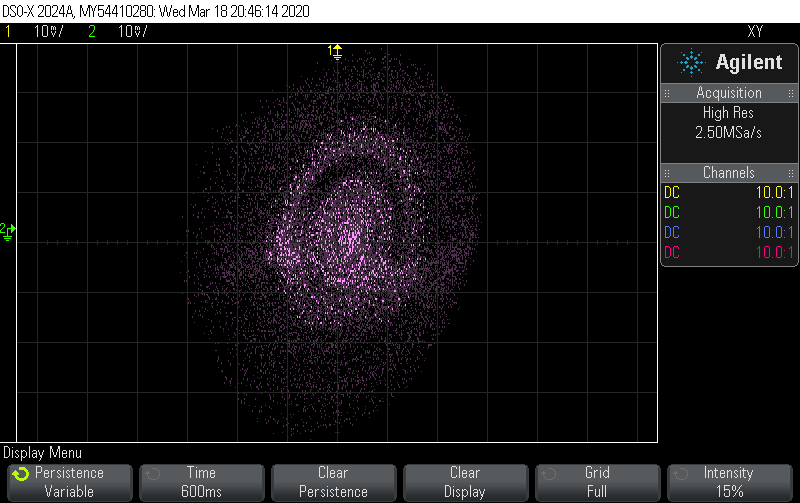
\includegraphics[trim={6cm 2cm 9cm 2cm},clip,width=\textwidth]{../imagenes/Y6p_Y_vs_Z.png}
	    \caption{$y$ vs $z$}
	    \label{Y6p_Y_vs_Z}
	  \end{subfigure}
	\end{figure}
	\end{frame}	
%%----------------------------------------------------------------------------------
%%----------------------------------------------------------------------------------
	\begin{frame}
		\frametitle{Oscilador caótico}
		\begin{figure}[!ht]
		\textbf{Topología de suma de filtros}
	\caption{Respuesta en el dominio temporal de oscilador caótico con $\alpha = 0.8$ y dos enrollamientos.}
	\label{fig:temporal_imp}
	  \begin{subfigure}[b]{0.3\textwidth}
	    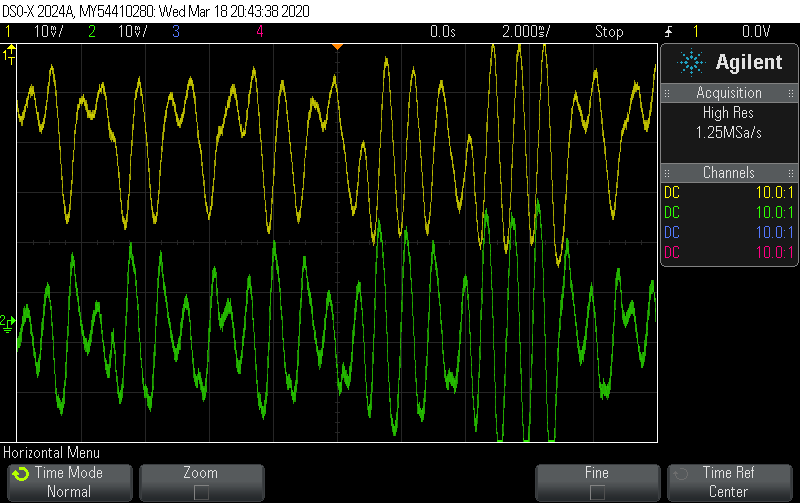
\includegraphics[trim={6cm 2cm 9cm 2cm},clip,width=\textwidth]{../imagenes/Y3p_X_vs_Y_signal.png}
	    \caption{$x$,$y$ respecto al tiempo.}
	    \label{fig:Y3p_X_vs_Y_signal}
	  \end{subfigure}
	  \hfill
	  \begin{subfigure}[b]{0.3\textwidth}
	    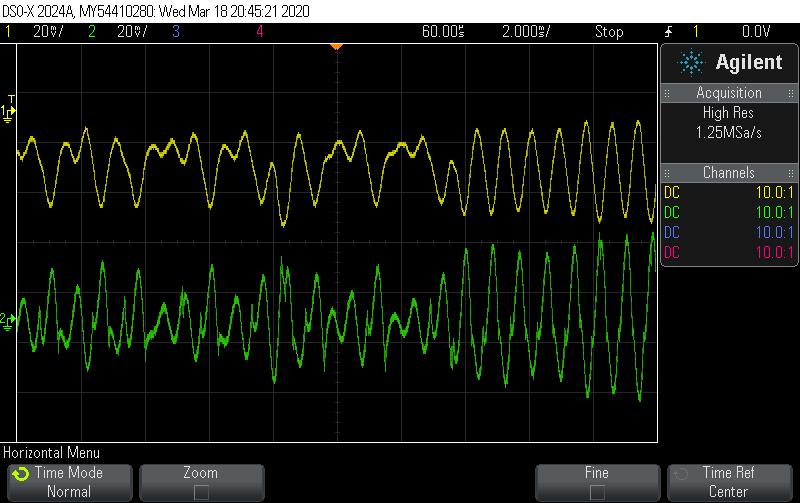
\includegraphics[trim={6cm 2cm 9cm 2cm},clip,width=\textwidth]{../imagenes/Y5p_X_vs_Z_signal.png}
	    \caption{$x$,$z$ respecto al tiempo.}
	    \label{fig:Y5p_X_vs_Z_signal}
	  \end{subfigure}
	  \hfill
	  \begin{subfigure}[b]{0.3\textwidth}
	    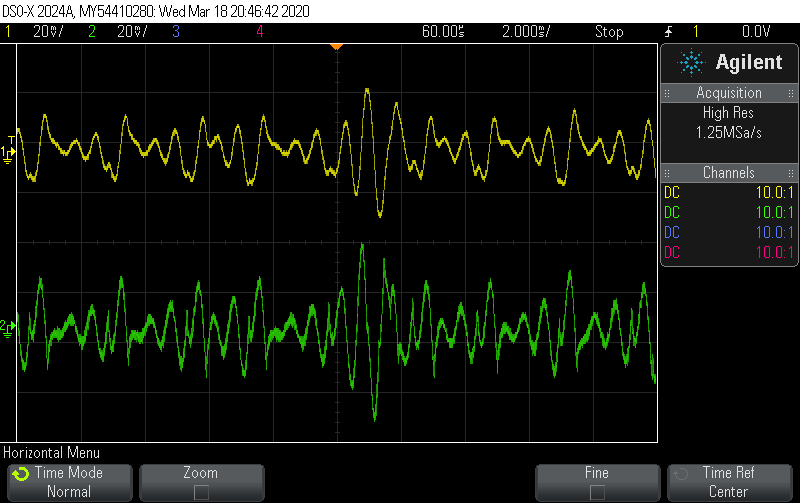
\includegraphics[trim={6cm 2cm 9cm 2cm},clip,width=\textwidth]{../imagenes/Y7p_Y_vs_Z_signal.png}
	    \caption{$y$,$z$ respecto al tiempo.}
	    \label{fig:Y7p_Y_vs_Z_signal}
	  \end{subfigure}
	\end{figure}	
	\end{frame}			
%%----------------------------------------------------------------------------------
%%----------------------------------------------------------------------------------
	\section{Conclusión}
	\begin{frame}
		\frametitle{Conclusión}
		\begin{block}{Conclusiones}
			\begin{itemize}
				\item 3 topologías de diseño para la síntesis de integradores fraccionarios.
					\begin{itemize}
						\item Primer orden con filtro bilineal pasabajas:
						\item Primer orden con suma de filtros bilineales, pasabajas y pasaaltas.
						\item Segundo orden con filtro bicuadrático
					\end{itemize}
				\item Integradores de orden fraccionario con rangos de [0.01, 0.93].
				
				\item Creación de metodologías de diseño en hardware y software:
				\begin{itemize}
					\item Conexiones y configuraciones del FPAA detalladas y simplificadas.
					\item Programas en MATLAB para generar tablas de diseño y gráficas de mérito.
				\end{itemize}
				\item Aplicaciones futuras:
					\begin{itemize}
						\item Controladores de orden fraccionario.
						\item Sistemas de encriptación.
					\end{itemize}
			\end{itemize}
		\end{block}
	\end{frame}	
	
	
	
	
	
	
	
	
	
	\section{Bibliografía}
	\begin{frame}[t, allowframebreaks]
		\frametitle{Bibliografía}
		\nocite{*}
		\bibliographystyle{ieeetr}
		\bibliography{bibliografia}
	\end{frame}
	
	\begin{frame}
		\frametitle{Introducción}
		\begin{block}{¿Qué es el caos?}
		\justifying
			El caos se refiere a un tipo de comportamiento dinámico complejo que posee algunas características muy especiales:
			\begin{itemize}
				\item Se describe mediante un conjunto de ecuaciones diferenciales ordinarias.
				\item Posee extrema sensibilidad a pequeñas variaciones.
				\item Presenta trayectorias encerradas en el espacio de fase.
			\end{itemize}
		\end{block}
	\end{frame}	
	
	
		\begin{frame}
		\frametitle{Introducción}
		\begin{block}{Aplicaciones de osciladores caóticos}
			\begin{itemize}
				\item Técnicas de modulación.
				\item Sistemas de comunicación.
				\item Encriptación de datos usando caos.
				\item Modelado de sistemas biológicos.
				\item Reacciones químicas.
				\item Toma de decisiones criticas en política, economía y eventos militares.
				\end{itemize}
		\end{block}

\begin{figure}[!h]
	\begin{minipage}[c]{0.45\textwidth}
		\centering
		
\includegraphics[width = 3.5cm]{encrypt.png}
%		\caption{Oscilador caótico de Chen de orden fraccionario.}
	\end{minipage} \hfill \begin{minipage}[c]{0.45\textwidth}
		\centering
		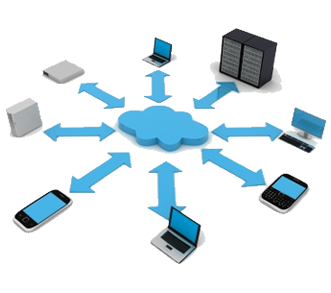
\includegraphics[width = 4cm]{comunication.png}
%		\caption{Oscilador caótico de Chen de orden fraccionario.}
	\end{minipage}
\end{figure}
	\end{frame}
	
	\begin{frame}
		\frametitle{Diagrama de bloques}
		\begin{figure}[hbtp]
			\centering
			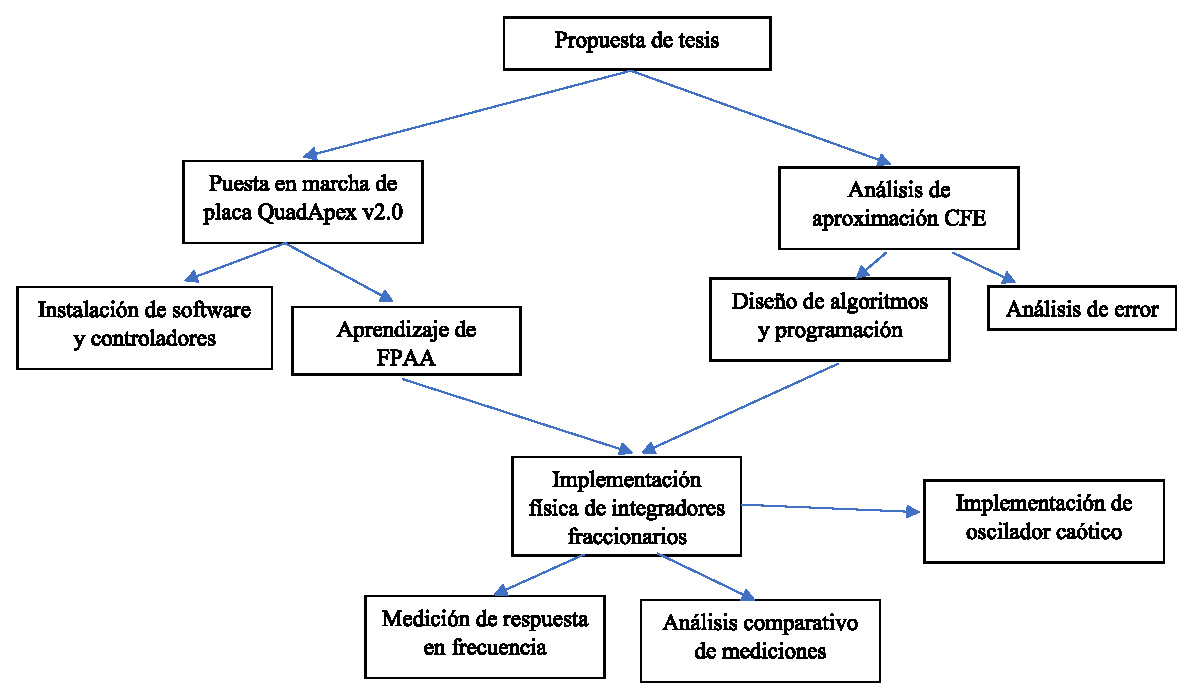
\includegraphics[width = 10cm]{diagrama_de_bloques.eps}
%			\caption{Atractor de oscilador caótico de Chen de orden fraccionario.}
		\end{figure}
	\end{frame}

%%----------------------------------------------------------------------------------
%%----------------------------------------------------------------------------------
	\begin{frame}
		\frametitle{Oscilador caótico}
		\begin{block}{ }
		\begin{table}[!ht]                                      
		\centering   
		\caption{Conexiones de DIP switches, jumpers y cables externos.}                            
		\label{tab:resumen_de_imp}                                       
			\begin{tabular}{c c c}                        
			\hline                                              
			Switch & Jumper & Cables externos\\            
			\hline       
			{\color{magenta} S$3$ $\quad2\downarrow$}& J8 & FPAA1 O3 $\rightarrow$ FPAA3 I5\\  
			{\color{magenta} S$5$ $\quad2\downarrow$}& J9& FPAA1 I5 $\rightarrow$ FPAA3 O5\\
			{\color{red} S$4$ $\quad2\uparrow$}&J10&\\ 
			{\color{red} S$6$ $\quad2\uparrow$}&ACT1 &\\
			{\color{blue} S$7$ $\quad2\uparrow$}& ACT2 &\\ 
			S12& ACT3 &\\ 
			S13& ACT4 &\\ 
			\hline                                 
			\end{tabular}                                                             
	\end{table}	
		\end{block}
	\end{frame}	



\end{document}